\chapter{Аутоматизација одлучивања}
\label{ch:automatizacija}

\section{Концепт и значај AI аутоматизације}

\subsection{Концепт и еволуција аутоматизације}

\subsubsection{Дефинисање савремене аутоматизације}

У савременој теорији менаџмента, теорије одлучивања и пракси информационих технологија, аутоматизација се више не посматра као бинарни процес замене људског рада машинским. Она представља софистицирану оркестрацију софтверских алата, података и алгоритама вештачке интелигенције (AI) са циљем оптимизације пословних процеса и прављења што бољих одлука.

Док је индустријска револуција донела аутоматизацију физичког рада (механизацију), дигитална револуција у којој се налазимо доноси аутоматизацију когнитивних процеса.

\begin{tcolorbox}[colback=gray!10!white,colframe=blue!50!black,title=Formalna definicija]
\textbf{AI Аутоматизација} (енг. \textit{Intelligent Process Automation - IPA}) дефинише се као примена напредних технологија, укључујући обраду природног језика (NLP), машинско учење (ML) и структуриране радне токове, ради извршавања задатака који су традиционално захтевали људску перцепцију и расуђивање~\cite{russell2020,goodfellow2016}.
\end{tcolorbox}

Суштинска разлика између традиционалног софтвера и AI аутоматизације лежи у \textbf{адаптибилности}. Традиционални софтвер захтева структуриране улазне податке (нпр. тачно попуњена поља у бази), док AI аутоматизација поседује способност разумевања неструктурираних података (нпр. слободан текст у емаилу, гласовна порука или слика).
На Слици~\ref{fig:04-1} приказана је визуелна разлика између индустријске аутоматизације, која се ослања на унапред програмиране и ригидне процесе, и AI аутоматизације, која уводи адаптивне системе засноване на учењу, аутономном доношењу одлука и сарадњи AI агената.

\begin{figure}[h!]
    \centering
    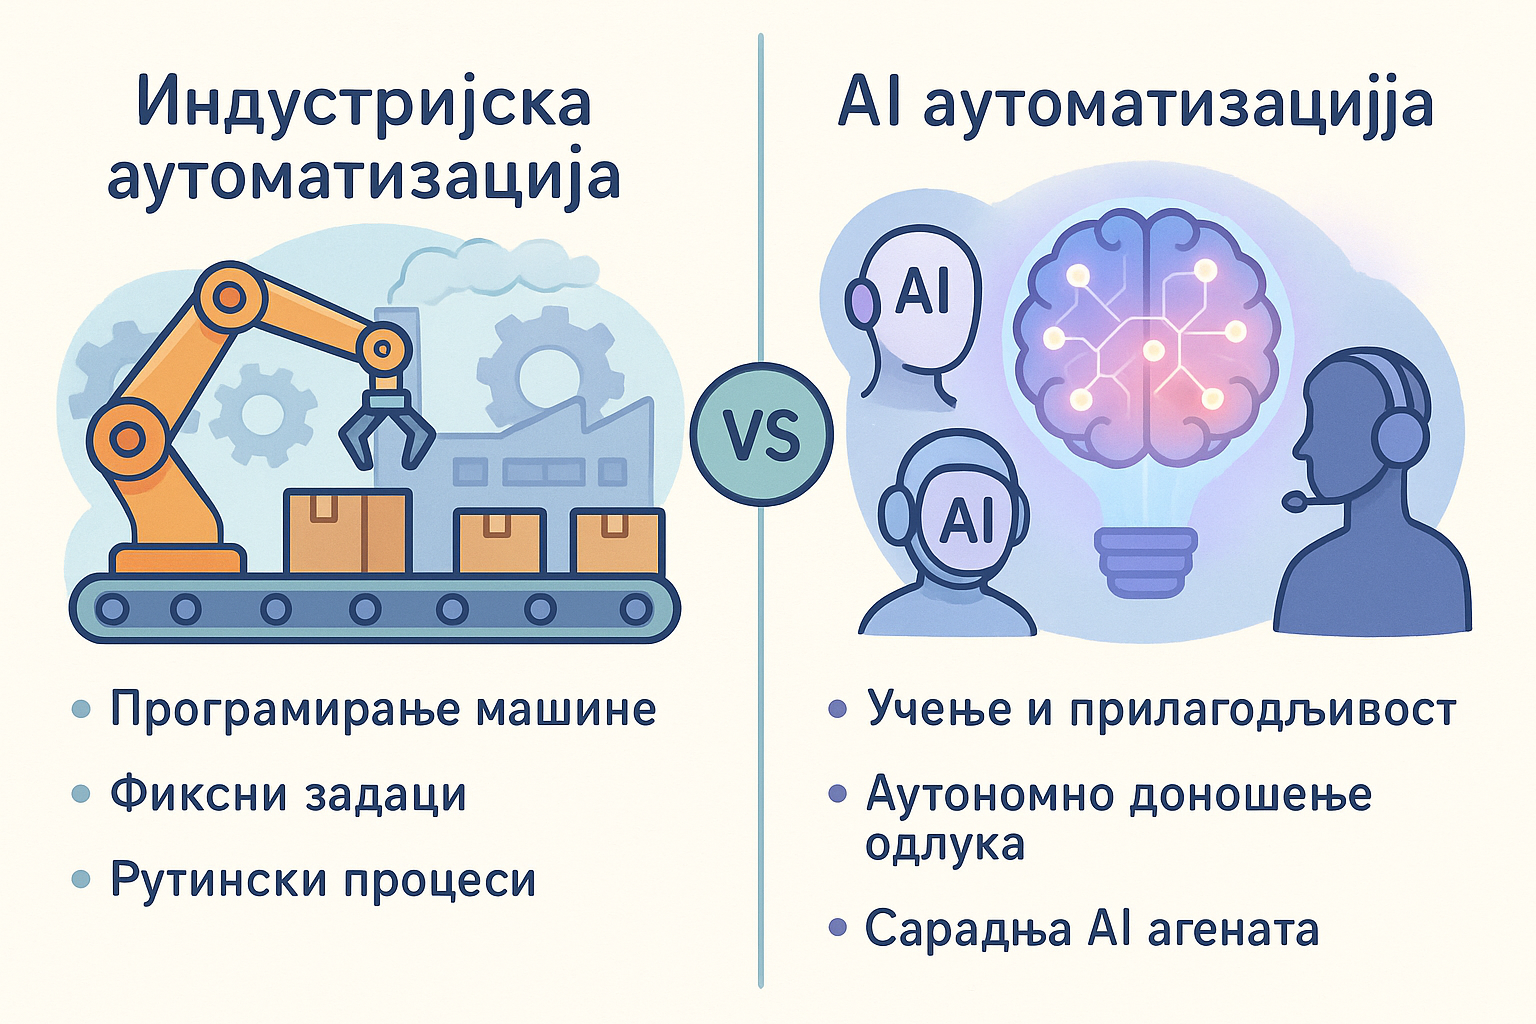
\includegraphics[width=0.95\textwidth]{slike/04/AI-Industrija.png}
    \caption{Поређење индустријске аутоматизације и AI аутоматизације}
    \label{fig:04-1}
\end{figure}

\subsubsection{Историјски развој: Од скрипти до когнитивних агената за одлучивање}

Да би се разумела тренутна парадигма, неопходно је сагледати еволутивни пут аутоматизације кроз три кључне фазе:

\begin{itemize}
    \item \textbf{Фаза 1: Скриптована аутоматизација (\textit{Scripting}).} \\
    Ово је најосновнији облик, резервисан за инжењере. Подразумева писање кода (Bash, Python, SQL) за извршавање једноставних, линеарних задатака (нпр. прављење резервне копије базе података сваке ноћи). Ови системи су ригидни; свака промена у окружењу доводи до прекида рада ("пуцања") скрипте.
    
    \item \textbf{Фаза 2: Роботска аутоматизација процеса (RPA).} \\
    RPA технологија омогућила је софтверу да имитира акције корисника на графичком интерфејсу (кликтање, куцање). Иако напреднија од скрипти, RPA и даље не разуме шта ради, већ само прати координате и правила. Ако се дугме на сајту помери за 5 пиксела, процес може стати~\cite{ivancic2019,wewerka2020rpa}.
    
    \item \textbf{Фаза 3: AI и Когнитивна аутоматизација (IPA).} \\
    Интеграцијом великих језичких модела (енг \textit{Large Language models - LLM})~\cite{brown2020,zhao2023llmsurvey}, аутоматизација добија способност "разумевања". Систем више не прати само координате, већ анализира семантичко значење. Ако се формат фактуре промени, AI агент и даље може препознати шта је нпр. датум, а шта износ, чинећи систем робусним и отпорним на промене.
\end{itemize}

Табела~\ref{tab:04-1} приказује кључне разлике између традиционалне аутоматизације засноване на правилима (RPA) и савремене AI аутоматизације. Традиционална аутоматизација функционише над строго структурираним подацима и ослања се на фиксна, унапред дефинисана правила, што је чини погодном за линеарне и понављајуће процесе са јасним улазно-излазним обрасцима. Такви системи су релативно једноставни за евалуацију, али захтевају интензивно одржавање, нарочито у случају промена пословних правила или структуре података.
Насупрот томе, AI аутоматизација је дизајнирана за рад са неструктурираним подацима, као што су текст, слике или глас, и карактерише је висока флексибилност захваљујући способности учења и прилагођавања. Ови системи уводе нелинеарне токове одлучивања и могу аутономно прилагођавати своје понашање на основу нових података и контекста. Иако такав приступ омогућава решавање знатно комплекснијих задатака, он истовремено отежава формалну евалуацију и захтева напредне методе валидације, интерпретабилности и надзора.


\begin{table}[h]
\centering
\caption{Компарација традиционалне и AI аутоматизације}
\vspace{0.3cm}
\begin{adjustbox}{max width=\textwidth}
\begin{tabular}{|p{5cm}|p{4.5cm}|p{4.5cm}|}
\hline
\textbf{Карактеристика} & \textbf{Традиционална (RPA)} & \textbf{AI Аутоматизација} \\
\hline
\textbf{Тип података} & Структурирани & Неструктурирани  \\
\hline
\textbf{Флексибилност} & Ниска (Фиксна правила) & Висока (Прилагодљива) \\
\hline
\textbf{Одржавање} & Захтевно  & Аутономно  \\
\hline
\textbf{Комплексност} & Линеарна & Нелинеарна \\
\hline
\textbf{Евалуација} & Лака & Тешка \\
\hline
\end{tabular}
\end{adjustbox}
\label{tab:04-1}
\end{table}

\subsubsection{"No-Code" револуција}

Један од најважнијих аспеката савремене аутоматизације, који се често наглашава у стручној литератури, јесте спуштање баријере уласка. До пре неколико година, изградња аутоматизованих агената захтевала је високо стручно знање из области софтверског инжењерства. Данас сведочимо успону тзв. \textbf{Citizen Developers} (Грађани-програмери). Захваљујући платформама као што су \textit{n8n}, \textit{Make} или \textit{Zapier}, процес програмирања је апстрахован кроз визуелне интерфејсе.

Уместо писања синтаксе кода, корисници креирају логику повезивањем визуелних блокова (чворова). Сваки чвор представља одређену функцију (нпр. „Прочитај email“, „Пошаљи Slack поруку“, „Питај ChatGPT“). Ово не значи да програмирање нестаје, већ да се фокус помера са \textit{sintakse} (како написати код) на \textit{logiku i arhitekturu} (шта систем треба да уради)~\cite{n8n,langchain}. Ово омогућава доменским експертима – људима из маркетинга, продаје, права или медицине – да сами граде алате који решавају њихове специфичне проблеме, без чекања на ИТ одељења.

\begin{quote}
\textit{"Аутоматизација више није алат за ИТ сектор, већ основна писменост модерног пословања у циљу прављења што бољих одлука."}
\end{quote}

Овај тренд доводи до брже итерације у пословању. Идеја се може претворити у функционалан прототип (MVP) за неколико сати, уместо за неколико недеља развоја, што радикално убрзава дигиталну трансформацију компанија. На слици~\ref{fig:04-2} задат је илустративни приказ "No-Code" револуције.

\begin{figure}[h!]
    \centering
    
\includegraphics[width=0.95\textwidth]{slike/04/nocode.png}
    \caption{"No-Code" револуција}
    \label{fig:04-2}
\end{figure}

% =================================================================================
% POGLAVLJE 1.2 - PROŠIRENA VERZIJA
% =================================================================================

\subsection{Стратешке предности имплементације аутоматизованих система}

Анализом савремених пословних процеса и студија случаја дигиталне трансформације, идентификован је низ стратешких и оперативних бенефита који произилазе из увођења AI аутоматизације. Ови бенефити превазилазе пуко смањење трошкова и дотичу се фундаменталне реорганизације начина на који се ствара вредност у компанији у циљу прављења што бољих одлука.

У наставку је дата детаљна анализа четири кључна стуба вредности аутоматизације.

\subsubsection*{1. Оперативна ефикасност и оптимизација људског капитала}

Најчешће помињан разлог за увођење аутоматизације је уштеда времена, међутим, у академском и менаџерском смислу, прецизније је говорити о \textbf{ре-алокацији когнитивних ресурса}.

У традиционалном моделу пословања, висококвалификовани запослени често троше између 30\% и 50\% свог радног времена на административне задатке ниске вредности (енг. \textit{Low-Value Tasks}), као што су:
\begin{itemize}
    \item Мануелни унос података из фактура у рачуноводствени софтвер.
    \item Копирање информација из емаилова у CRM системе.
    \item Организација састанака и усклађивање календара.
    \item Генерисање рутинских недељних извештаја.
\end{itemize}

Имплементацијом AI агената, ови процеси се делегирају машини. Ово доводи до феномена познатог као \textbf{"Когнитивно растерећење"} (\textit{Cognitive Offloading}). Када се запослени ослободи репетитивних радњи, његови капацитети се преусмеравају на послове високе вредности (енг. \textit{High-Value Work}):
\begin{itemize}
    \item Стратешко планирање: Анализа тржишних трендова и дефинисање дугорочних циљева.
    \item Креативно решавање проблема: Иновација производа и услуга.
    \item Емоционални рад: Изградња дубљих односа са кључним клијентима и управљање тимовима.
\end{itemize}

На основу наведеног може се извести једноставан закључак:
\begin{quote}
\textit{Економски посматрано, аутоматизација повећава повраћај на инвестицију (ROI) по запосленом, јер се цена радног сата човека троши на задатке које само човек може да обави, односно задатке које захтевају додатан интелектуални напор}
\end{quote}

\subsubsection*{2. Минимизација људске грешке и интегритет података}

Људски фактор је, статистички гледано, најслабија карика у процесима обраде података. Истраживања показују да при мануелном уносу података стопа грешке (типо, изостављање, погрешно поље) износи између 1\% и 4\%~\cite{vanderaalst2016}. Иако делује мало, у системима који обрађују хиљаде трансакција, ово доводи до значајних финансијских губитака и оперативних застоја.

Аутоматизовани системи уводе концепт \textbf{детерминистичког извршења}. То значи да ће софтверски агент, под истим условима, увек извршити задатак на идентичан начин.

Предности оваквог приступа су вишеструке:
\begin{itemize}
    \item \textbf{Конзистентност:} Податак који се аутоматски преноси из CRM система у ERP биће идентичан у 100\% случајева.
    \item \textbf{Усклађеност:} Аутоматизовани токови остављају дигитални траг (енг. \textit{Log files}). У индустријама попут банкарства или здравства, ово је кључно за ревизију и поштовање регулатива (као што је GDPR). Тачно се зна ко је (који агент), када и како обрадио податак.
    \item \textbf{Финансијска сигурност:} Елиминација грешака у фактурисању или обрачуну плата директно спречава одлив новца.
\end{itemize}

\subsubsection*{3. Скалабилност и еластичност пословања}

Један од највећих изазова за растуће компаније је тзв. "кочница људских ресурса". У мануелном моделу, раст обима посла линеарно прати раст трошкова радне снаге.
$$
\text{Обим посла} \uparrow \;\approx\; \text{Број запослених} \uparrow \;\approx\; \text{Трошкови} \uparrow
$$
Аутоматизација разбија ову линеарну зависност и омогућава експоненцијалну скалабилност. Софтверска инфраструктура поседује еластичност коју људска радна снага нема.

\textbf{Примери скалабилности:}
\begin{enumerate}
    \item \textbf{Управљање пиковима (Spikes):} Током периода као што је „Black Friday“, број упита корисника може порасти за 1000\%. Људски тим би био преплављен, што би довело до пада квалитета услуге. AI агенти могу тренутно скалирати своје капацитете (уз минимално повећање трошкова сервера) како би обрадили сав саобраћај без кашњења.
    \item \textbf{Микро-скалирање:} За мале бизнисе, аутоматизација омогућава да једна особа управља процесима за које би иначе био потребан тим од петоро људи (продаја, маркетинг, подршка, финансије).
\end{enumerate}

Ово омогућава компанијама да расту приходе много брже него што расту оперативни трошкови, чиме се повећава профитна маржа.

\subsubsection{Континуитет пословања (Концепт "Always-On")}

У глобалној дигиталној економији, концепт радног времена (9-до-5) постаје застарео. Потрошачи очекују инстант гратификацију и одговоре у реалном времену, без обзира на временску зону.

За разлику од биолошке радне снаге, дигитални радници (AI Агенти):
\begin{itemize}
    \item Не захтевају сан, одмор или паузе за ручак.
    \item Нису подложни паду концентрације услед замора.
    \item Не одлазе на боловања или годишње одморе.
\end{itemize}

Ово омогућава успостављање \textbf{континуитета пословања 24/7/365}.

\textbf{Практична импликација:}
Клијент из друге временске зоне (нпр. САД) може послати упит локалној фирми (нпр. у Србији) у 3 сата ујутру. Уместо да чека до 9 ујутру да запослени дође на посао, AI агент може:
\begin{enumerate}
    \item Тренутно анализирати упит.
    \item Проверити базу знања.
    \item Послати релевантан одговор или решити проблем (нпр. ресетовање лозинке).
    \item Заказати састанак у слободном термину запосленог за следећи дан.
\end{enumerate}

Резултат је драстично повећање задовољства корисника (енг. \textit{Customer Satisfaction}) и брже затварање продајних циклуса.


\subsection{Конзистентност и аналитика}

Аутоматизација намеће стандардизацију. Да би се процес аутоматизовао, он прво мора бити јасно дефинисан. Ово доводи до стварања конзистентних система који не зависе од индивидуалних навика запослених.

Додатно, аутоматизовани системи генеришу велику количину метаподатака. Уместо ручног прикупљања извештаја, менаџмент добија увид у перформансе система у реалном времену (енг. \textit{Real-time insights}), што омогућава доношење одлука заснованих на подацима (енг. \textit{Data-driven decision making}).

\subsection{Доменске области примене (\textit{Use Cases})}

Свестраност технологије AI аутоматизације омогућава њену имплементацију у готово свим порама модерног пословања. Ипак, анализа тржишта показује да се највећи повраћај на инвестицију (ROI) остварује у пет кључних пословних функција.

У наставку је дата детаљна дисекција примене аутоматизованих агената у овим вертикалама, са фокусом на трансформацију процеса из мануелних у аутономне.

\paragraph*{Продаја и управљање односима са клијентима (CRM)}
\noindent
CRM (енг. \textit{Customer Relationship Management}) системи представљају срце продајних организација, али су често неефикасни услед лошег квалитета података и неажурности продаваца. AI аутоматизација решава проблем шумовитих података и убрзава продајни циклус.

\begin{itemize}
    \item \textbf{Обогаћивање података о лидовима (Lead Enrichment):} \\
    Када корисник остави само емаил адресу на сајту, AI агент може аутоматски претражити јавне базе (LinkedIn, компанијске регистре), прикупити податке о позицији, величини фирме и индустрији, и ажурирати CRM профил пре него што продавац уопште види контакт.
    
    \item \textbf{Интелигентно бодовање лидова (AI Lead Scoring):} \\
    Уместо субјективне процене, алгоритми анализирају понашање корисника (отварање мејлова, посета страници са ценама) и аутоматски додељују приоритет~\cite{raffel2020t5,wolf2020transformers}. Агенти могу аутоматски заказати састанак само са оним клијентима који имају високу вероватноћу куповине, док остале стављају у процес едукације (nurturing).
    
    \item \textbf{Аутоматизовани Follow-up:} \\
    Статистика показује да је потребно просечно 5 до 7 контаката да би се закључила продаја. Људи често одустану након другог. AI агенти могу неуморно слати персонализоване секвенце порука (путем Емаил-а, LinkedIn-а или WhatsApp-а) све док не добију одговор, драстично повећавајући стопу конверзије.
\end{itemize}

\paragraph*{Корисничка подршка и искуство (Customer Support)}
\noindent
Ово је област где је примена AI највидљивија. Прелазак са класичних call-центара на хибридне AI системе мења парадигму подршке.

\begin{itemize}
    \item \textbf{Агенти првог нивоа (L1 Support):} \\
    AI агенти, оснажени RAG (енг. \textit{Retrieval Augmentation Generation}) архитектуром~\cite{lewis2020rag,gao2024ragsurvey}, могу решити између 60\% и 80\% рутинских упита (статус поруџбине, повраћај новца, основна техничка питања) без интервенције човека. За разлику од старих „chatbot-ова“ са фиксним менијима, ови агенти разумеју природни језик и контекст.
    
    \item \textbf{Анализа сентимента и приоритизација:} \\
    Приликом пријема тикета, AI анализира тон поруке. Ако детектује фрустрацију или бес ("Љутит клијент"), систем аутоматски ескалира тикет директно менаџеру подршке, заобилазећи стандардну процедуру чекања.
    
    \item \textbf{Omnichannel синхронизација:} \\
    Агенти прате интеракције на свим каналима. Ако се корисник жалио на Twitter-у, а затим послао емаил, систем препознаје да је то иста особа и исти проблем, омогућавајући агенту подршке увид у комплетну историју комуникације.
\end{itemize}

\paragraph{Маркетинг операције и генерисање садржаја}
\noindent
Маркетинг је еволуирао из креативне у техничко-креативну дисциплину. Аутоматизација омогућава хипер-персонализацију на скали коју људи не могу постићи.

\begin{itemize}
    \item \textbf{Генерисање и варијација садржаја:} \\
    Коришћењем генеративних модела, аутоматизација може креирати стотине варијација огласа (текст и слика) прилагођених различитим циљним групама. Агент може написати блог пост, затим га аутоматски претворити у LinkedIn објаву, Twitter низ (thread) и скрипту за TikTok видео.
    
    \item \textbf{Системи препоруке:} \\
    Уместо слања истог newsletter-а свима, систем аутоматски сегментира базу на основу понашања. Ако је корисник кликнуо на линк о „AI алатима“, аутоматски улази у секвенцу која му шаље више садржаја на ту тему.
    
    \item \textbf{Social Listening и реакција:} \\
    AI агенти могу 24/7 пратити помињање бренда на интернету. У случају негативног помињања, могу алармирати PR тим, или у случају позитивног, аутоматски лајковати и захвалити се кориснику.
\end{itemize}

\paragraph{Финансијски менаџмент и рачуноводство}
\noindent
Финансијски сектор захтева прецизност и усклађеност са прописима, што га чини идеалним кандидатом за детерминистичку аутоматизацију.

\begin{itemize}
    \item \textbf{Аутоматизација обраде фактура (Accounts Payable):} \\
    AI агенти користе OCR (енг. \textit{Optical Character Recognition}) да прочитају PDF фактуре које стижу на емаил, екстрахују податке (добављач, износ, ПИБ), провере да ли се слажу са наруџбеницом и аутоматски их унесу у рачуноводствени софтвер или припреме налог за плаћање~\cite{schwab2017}.
    
    \item \textbf{Упаривање трансакција (Reconciliation):} \\
    Упоређивање банковних извода са интерним књиговодством је мукотрпан процес. Аутоматизација може у секундама упарити хиљаде ставки и издвојити само оне које се не слажу (аномалије) за људску ревизију.
    
    \item \textbf{Управљање трошковима:} \\
    Запослени могу сликати рачун телефоном, а AI агент аутоматски категоризује трошак, проверава да ли је у складу са политиком фирме и шаље на одобрење.
\end{itemize}

\paragraph{Управљање пројектима и HR процеси}

Интерна ефикасност организације директно зависи од брзине протока информација.

\begin{itemize}
    \item \textbf{Аутоматизовани Onboarding запослених:} \\
    Када се у HR систему означи да је нови запослени примљен, агент аутоматски: креира email налог, додаје га у релевантне Slack канале, шаље уговор на потписивање, заказује уводне састанке и шаље материјале за обуку.
    
    \item \textbf{Праћење статуса пројеката:} \\
    Уместо дугих састанака за „статус update“, AI агент може на крају дана питати сваког члана тима „Шта си данас урадио?“ путем chat-а, сумирати све одговоре и послати менаџеру консолидовани извештај о напретку пројекта.
\end{itemize}


\newpage

% =================================================================================
% POGLAVLJE 2
% =================================================================================

\section{Техничка инфраструктура аутоматизације}
\label{sec:tehnicka-infrastruktura}

У претходном поглављу разматрани су концептуални и стратешки аспекти AI аутоматизације, са фокусом на пословну вредност,
доменске примене и организационе импликације. Међутим, како би аутоматизација прешла из теоријског оквира у реалну,
продукцијску примену, неопходно је детаљно разумети техничку инфраструктуру која такве системе чини могућим.

Техничка инфраструктура аутоматизације представља скуп међусобно повезаних софтверских компоненти које омогућавају:
детекцију догађаја, оркестрацију процеса, размену података између хетерогених система, доношење интелигентних одлука
и надзор над извршавањем у реалном времену~\cite{omg2014bpmn,vanderaalst2016}. За разлику од класичних информационих система, где су токови често
тврдо кодирани и монолитни, савремени аутоматизовани системи су дистрибуирани, догађајима вођени и високо модуларни.

Посебан изазов у пројектовању оваквих система представља интеграција компоненти вештачке интелигенције.
AI модели, нарочито велики језички модели, нису детерминистички по својој природи и не могу се посматрати као
једноставна замена за традиционални програмски код. Због тога је неопходно увести јасну архитектонску структуру
у којој AI функционише као контролисана и надзирана компонента унутар ширег аутоматизованог тока.

У овом поглављу биће представљена референтна техничка архитектура AI аутоматизације, као и кључни инфраструктурни
концепти који омогућавају њену поуздану, скалабилну и безбедну примену у пракси. Посебан акценат биће стављен
на улогу оркестрације, интеграција, управљања подацима и обсервабилити слоја, уз илустрацију кроз савремене
workflow алате који омогућавају визуелно моделовање комплексних процеса.


\subsection{Референтна архитектура аутоматизације}
\label{sec:ref_arch}

Техничка инфраструктура AI аутоматизације може се посматрати као слојевита архитектура која комбинује:
(и) механизме за \textit{детекцију догађаја} (тригери), (ии) систем за \textit{orkestraciju toka rada} (workflow engine),
(иии) интеграције са спољним сервисима путем API-ја, (ив) слој за управљање подацима, и (в) AI слој који доноси
одлуке и генерише садржај на основу контекста.

У пракси, ове компоненте не чине монолит, већ модуларан систем у коме се сваки слој може независно заменити
или унапредити. Такав приступ је кључан за одрживост аутоматизације: процеси се временом мењају, уводе се нови алати,
а промена једног сервиса (нпр. CRM система) не би смела да уруши читав аутоматизовани ток.

\subsubsection{Слојеви референтне архитектуре}

У наставку су описани основни слојеви референтне архитектуре аутоматизације. Сваки слој представља логичку целину,
док се у имплементацији често преклапају или спајају у зависности од величине система.

\paragraph*{1. Trigger слој (иницирање процеса)}
Trigger слој је улазна тачка аутоматизације: он детектује догађај и покреће ток рада. Типични окидачи су:
\begin{itemize}
    \item \textbf{Ручни тригер:} ово представља ручни тригер за окидање и извршавање тока рада.
    \item \textbf{Webhook догађаји:} нпр. нова поруџбина у web shop-у или нова пријава кроз форму.
    \item \textbf{Scheduler (временски окидач):} нпр. стартовање тока рада сваког понедељка у 08:00.
    \item \textbf{Inbox / поруке / чет порука:} нпр. пријем емаила у специфично сандуче, нова порука у chat каналу.
    \item \textbf{Системски догађаји:} нпр. промена у бази података или нови фајл у фолдеру (Google Drive trigger).
\end{itemize}

У индустријским системима, начин иницирања процеса директно утиче на латенцију и поузданост~\cite{airflow}.
Webhook приступ омогућава реакцију у реалном времену, док scheduler и ручни тригери имају веће кашњење,
али могу бити једноставнији за имплементацију у окружењима где webhook-ови нису доступни. На слици~\ref{fig:04-3} задат је илустративни приказ тригера у \textit{n8n} .

\begin{figure}[h!]
    \centering
    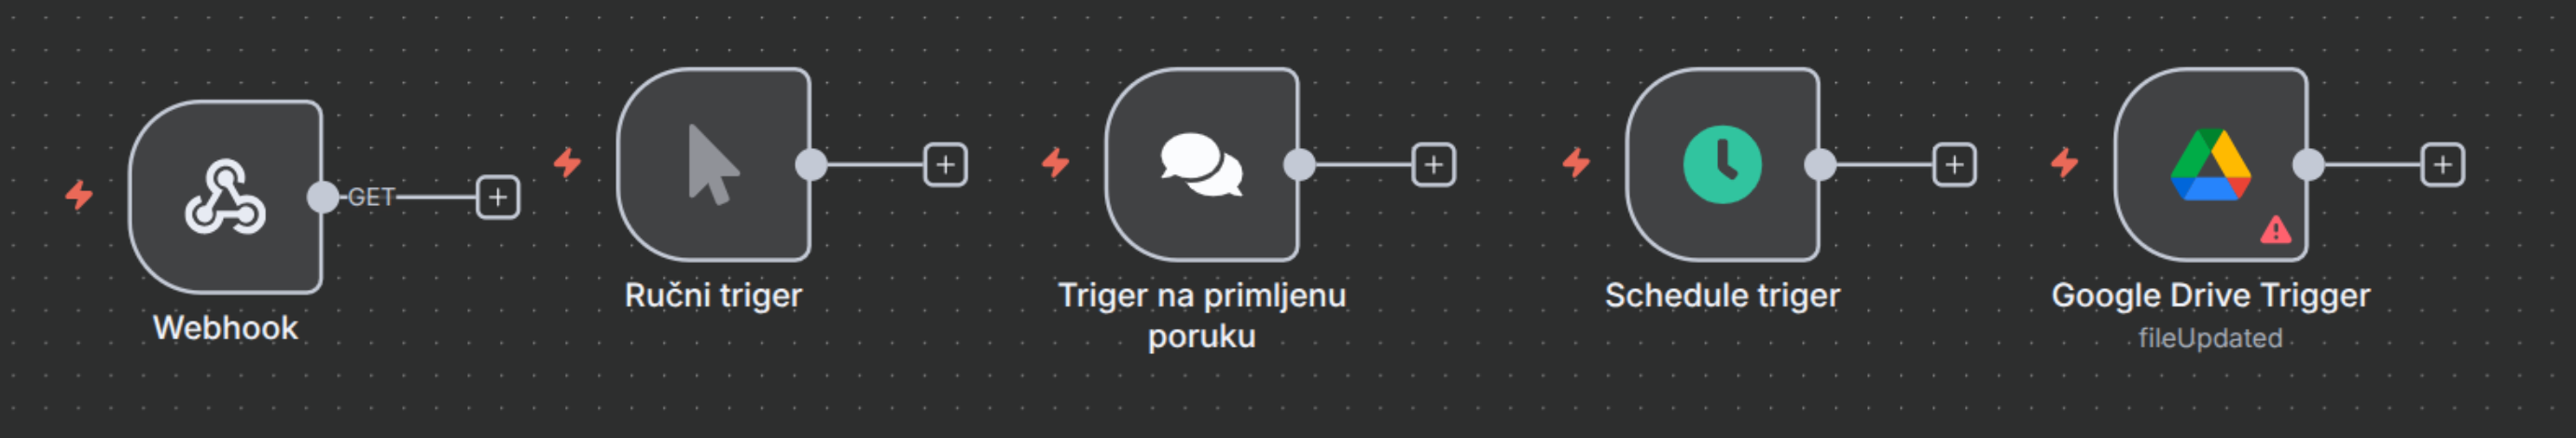
\includegraphics[width=0.95\textwidth]{slike/04/Trigeri.png}
    \caption{Илустративан приказ тригер иконица у \textit{n8n}}
    \label{fig:04-3}
\end{figure}

\paragraph*{2. Orchestration слој (workflow engine)}
Оркестрациони слој је \textit{centralni dirigent} аутоматизације. Његова улога је да:
\begin{itemize}
    \item управља редоследом корака (секвенца),
    \item доноси одлуке о гранању (иф/свитцх),
    \item координира паралелне активности,
    \item имплементира ретри/бацкофф када дође до грешке,
    \item чува контекст извршавања (нпр. \textit{run id}, стање процеса),
    \item логује резултате и грешке по корацима.
\end{itemize}

Генерално оркестрација се често демонстрира кроз алате типа \textit{n8n}, где су кораци представљени чворовима
који се повезују у граф процеса. Међутим, важно је нагласити да је оркестрација концептуално независна од алата:
workflow engine може бити и цустом микросервис, платформа или чак сет серверлесс функција повезаних догађајима~\cite{airflow,omg2014bpmn}. На слици~\ref{fig:04-4} задат је илустративни приказ тригера у \textit{n8n} .

\begin{figure}[h!]
    \centering
    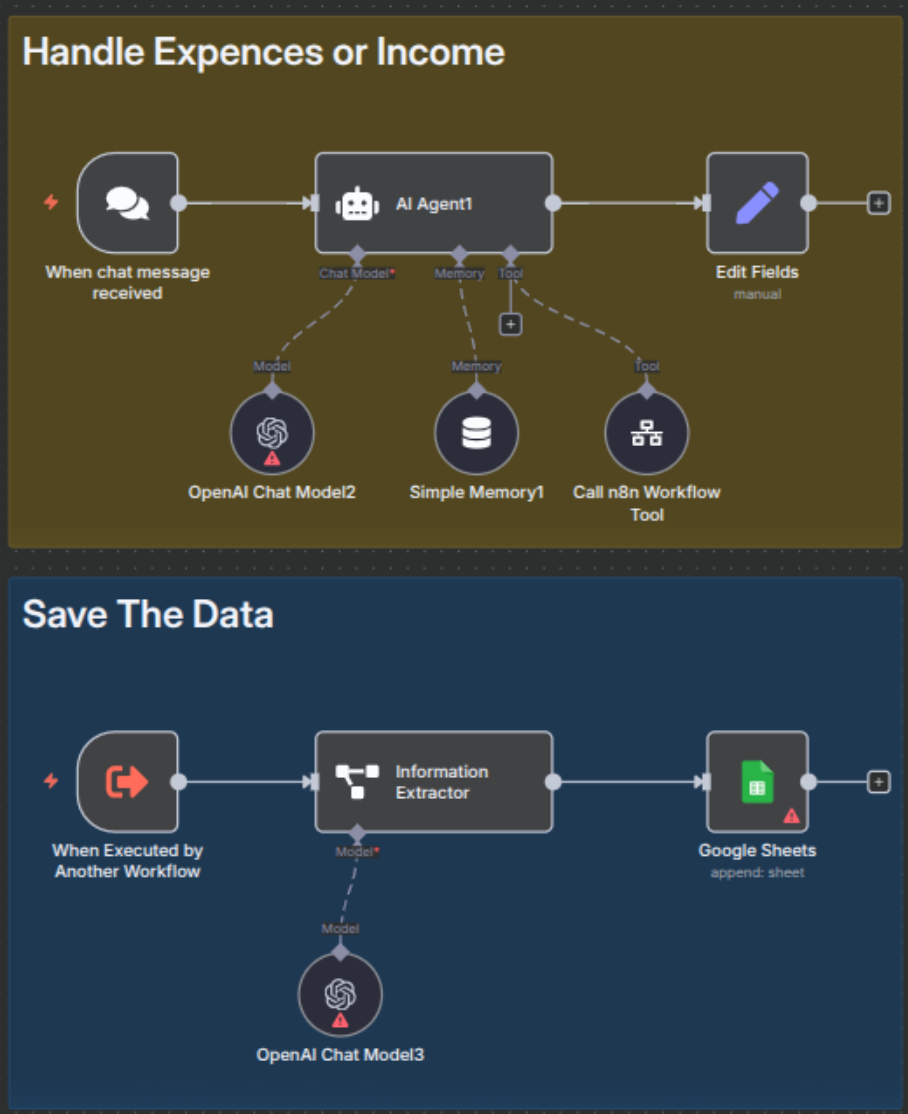
\includegraphics[width=0.8\textwidth]{slike/04/workflow_example.png}
    \caption{Илустративан приказ тока рада у \textit{n8n}}
    \label{fig:04-4}
\end{figure}


\paragraph*{3. Интеграциони слој (конектори и API комуникација)}
Интеграциони слој представља \textbf{спојно ткиво} аутоматизованог система и његовог спољног окружења.
Његова основна улога је да омогући поуздану, сигурну и стандардизовану размену података између аутоматизованог
workflow-а и различитих софтверских система који учествују у пословном процесу. Ови системи могу бити интерни
(CRM, ERP, базе података) или екстерни (паимент процесори, SaaS алати, државне платформе, аналитички сервиси).

У савременим информационим системима интеграција се готово искључиво ослања на API-је
(енг. \textit{Application Programming Interfaces}), који дефинишу како један софтверски систем излаже своје функционалности
другима. Аутоматизовани агент у том контексту преузима улогу клијента који шаље захтеве, прима одговоре и
тумачи их у складу са пословном логиком.

\paragraph*{Типови интеграционих интерфејса}

Најзаступљенији облик интеграције је \textbf{REST API}, где се размена података одвија путем HTTP протокола,
а операције су мапиране на стандардне HTTP методе:
\begin{itemize}
    \item \texttt{GET} – дохват података,
    \item \texttt{POST} – креирање нових записа или покретање акција,
    \item \texttt{PUT/PATCH} – измена постојећих записа,
    \item \texttt{DELETE} – брисање ресурса.
\end{itemize}

Поред REST-а, у одређеним доменима користе се и:
\begin{itemize}
    \item \textbf{GraphQL API}: омогућава флексибилно дефинисање тачно оних поља која су потребна,
    чиме се смањује количина пренетих података и број захтева.
    \item \textbf{SOAP сервиси}: и даље присутни у банкарским и државним системима, са строго дефинисаним шемама (WSDL).
    \item \textbf{SDK-ови и проприетарни интерфејси}: библиотеке које врше директну комуникацију са специфичним сервисима.
\end{itemize}

У контексту аутоматизације, избор интерфејса директно утиче на комплексност workflow-а, латенцију
и могућност детекције грешака.
У пракси, ови интерфејси се у оквиру аутоматизованих система често реализују кроз визуелне оркестрационе алате,
као што је \textit{n8n}, где је сваки API позив енкапсулиран у посебан чвор (ноде).
Такви чворови апстрахују нисконивојске детаље комуникације (HTTP методе, заглавља, аутентификацију),
док пројектанту процеса остављају фокус на логику тока, обраду одговора и руковање грешкама.
На овај начин, комплексне интеграције између хетерогених система могу се моделовати, тестирати и мењати
без потребе за писањем опсежног програмског кода, што значајно убрзава развој и одржавање аутоматизованих workflow-а.



\paragraph*{4. Дата слој (управљање подацима и меморија система)}
Дата слој обезбеђује да аутоматизација има стабилан ослонац у подацима. У најједноставнијем случају,
то може бити једна релациона база. У напредним системима разликују се најмање четири типа складишта:
\begin{itemize}
    \item \textbf{Оперативна база (OLTP):} нпр. PostgreSQL за трансакционе податке.
    \item \textbf{Документ складиште:} нпр. NoSQL база или фајл стораге за неструктуриране документе (PDF, слике).
    \item \textbf{Аналитичко складиште (OLAP):} агрегације, извештаји и БИ.
    \item \textbf{Векторска база:} складиштење embedding-а ради семантичке претраге (RAG системи)~\cite{johnson2019faiss,reimers2019sbert}.
\end{itemize}

Улога дата слоја је двострука: (и) чување резултата процеса (нпр. упис у CRM) и (ии) обезбеђивање контекста
за одлучивање (нпр. историја поруџбина клијента, правила, претходне комуникације). Дата слој је неопходан како би се агенти потхрањивали подацима. Примери чворова који представљају дата слој у \textit{n8n} дати су на слици~\ref{fig:04-5} 

\begin{figure}[h!]
    \centering
    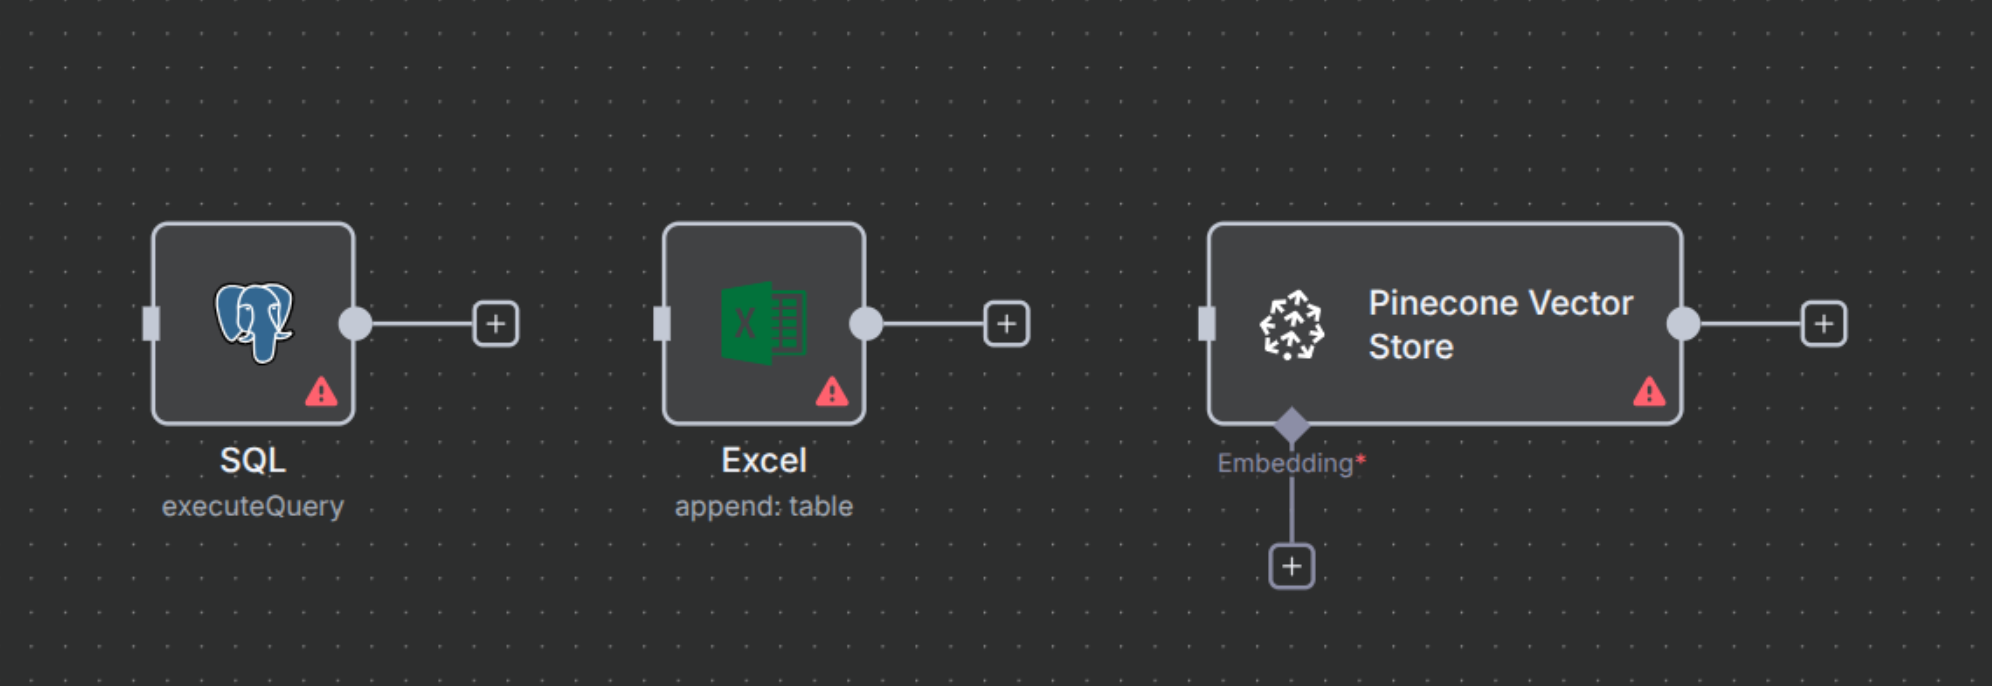
\includegraphics[width=0.8\textwidth]{slike/04/DB.png}
    \caption{Илустративан приказ тока рада у \textit{n8n}}
    \label{fig:04-5}
\end{figure}

\paragraph*{5. AI слој (модели, одлуке и генерисање)}
AI слој уводи способности које класична аутоматизација нема: разумевање текста, класификацију намере,
екстракцију информација из докумената, генерисање одговора и препорука~\cite{zhao2023llmsurvey}.

Типичне компоненте AI слоја укључују:
\begin{itemize}
    \item \textbf{LLM модели:} генерисање текста, сумирање, класификација и tool-calling~\cite{brown2020,schick2023toolformer}.
    \item \textbf{Embedding модели:} претварање текста/докумената у векторе за семантичку претрагу~\cite{mikolov2013,reimers2019sbert}.
    \item \textbf{OCR/VLM модели:} рад са сликама и документима (фактуре, уговори, формулари), као и \textit{Speech-to-Text} модели за обраду гласа~\cite{radford2022whisper}.
    \item \textbf{RAG архитектура:} комбиновање претраге знања и генерисања одговора~\cite{lewis2020rag}.
\end{itemize}
\noindent
Важно је нагласити да AI слој није замена за оркестрацију и интеграције, већ функционише као \textit{inteligentna komponenta}
унутар већег детерминистичког процеса. У добро пројектованом систему, AI делује унутар јасно дефинисаних граница:
добија контролисани input, генерише структурисан output, и пролази кроз валидацију пре него што утиче на спољашњи свет.

\paragraph*{6. Guardrails и контрола (валидација, сигурност и усклађеност)}

Како аутоматизација постепено преузима оперативне и одлучивачке задатке
(нпр. слање екстерних комуникација, креирање налога, иницирање финансијских трансакција),
неопходно је увести слој контроле који ограничава понашање система и спречава нежељене или
штетне последице~\cite{bai2022,hleg2019}. Овај слој, познат као \textbf{Guardrails}, представља скуп техничких и
организационих механизама који дефинишу границе дозвољеног деловања аутоматизованих агената. За разлику од класичних софтверских система, код којих је понашање детерминистички дефинисано
програмским кодом, системи засновани на вештачкој интелигенцији, а нарочито на великим језичким
моделима (LLM), производе генеративни излаз који може варирати у зависности од контекста.
Због тога контрола оваквих система захтева вишеслојни приступ.

\paragraph{Валидација излаза и структурална контрола}

Први ниво заштите односи се на проверу да ли је излаз система у складу са очекиваним форматом
и пословним правилима. У пракси се често користи:
\begin{itemize}
    \item валидација према унапред дефинисаним шемама (нпр. JSON Schema),
    \item провера типова података, опсега вредности и обавезних поља,
    \item одбацивање или корекција излаза који не задовољавају формалне критеријуме.
\end{itemize}

Овим приступом се спречава да генеративни модел произведе синтактички исправан, али
структурно неупотребљив или опасан резултат.

\paragraph{Политике понашања и домен дозвољених одговора}

Други ниво контроле чине експлицитне \textbf{политике и правила понашања}.
Оне дефинишу:
\begin{itemize}
    \item које врсте акција агент сме да изврши (нпр. слање информативних, али не и правно обавезујућих порука),
    \item на која питања сме да даје одговоре, а на која мора да одбије или ескалира захтев,
    \item границе доменског знања у оквиру којих агент може аутономно деловати.
\end{itemize}

У пословним системима, ове политике су често усклађене са интерним правилницима,
регулаторним захтевима и етичким смерницама организације.

\paragraph{Заштита осетљивих података и усклађеност}

Аутоматизовани системи често обрађују личне и поверљиве информације.
Због тога је маскирање и контрола осетљивих података (енг. \textit{Personally Identifiable Information -- PII})
од кључног значаја. Типичне мере укључују:
\begin{itemize}
    \item анонимизацију или псеудонимизацију података пре слања AI моделу,
    \item уклањање осетљивих информација из логова и промптова,
    \item строго ограничавање приступа подацима у складу са принципом најмањих привилегија,
    \item одбрану од индиректних напада кроз промпт-ињекцију, где злонамерни садржај у дохваћеним документима преусмерава понашање агента~\cite{greshake2023injection}.
\end{itemize}

Ове мере омогућавају усклађеност са регулативама као што су GDPR и интерне политике безбедности.

\paragraph{Human-in-the-loop и ескалација}

За акције са потенцијално високим ризиком (нпр. финансијске трансакције, раскид уговора,
слање правно осетљивих порука), аутоматизација се не ослања искључиво на аутономне одлуке.
Уместо тога, уводи се концепт \textbf{Human-in-the-loop}, где:
\begin{itemize}
    \item систем припрема предлог одлуке или акције,
    \item човек врши финалну проверу и одобрење,
    \item одлука се затим извршава или одбацује.
\end{itemize}

Овакав приступ комбинује ефикасност аутоматизације са одговорношћу и проценом човека.

\noindent
Закључно, Guardrails слој је кључни предуслов за безбедну и поуздану примену AI аутоматизације.
Он обезбеђује да интелигентни системи остану под контролом, чак и у ситуацијама непредвиђеног
понашања модела или промена у контексту.

\paragraph*{7. Опсервациони слој (логови и метрике)}

Без адекватног увида у рад система, аутоматизација постаје нетранспарентна,
тешка за одржавање и непоуздана у продукционом окружењу.
Observability слој омогућава континуирано праћење понашања аутоматизованих токова рада
и представља основ за дијагностику, оптимизацију и дугорочну стабилност система.

За разлику од класичног мониторинга, који се фокусира на основне показатеље доступности,
обсервабилити тежи разумевању \textit{зашто} је систем у одређеном стању.

\paragraph{Логовање извршавања}

Логови представљају хронолошки запис извршавања аутоматизованог процеса.
У контексту AI аутоматизације, логовање обухвата:
\begin{itemize}
    \item улазне податке и излазе по кораку workflow-а,
    \item статус извршења (успех, грешка, ретри),
    \item контекстуалне информације (време, идентификатор процеса).
\end{itemize}
\noindent
Како логови могу садржати осетљиве податке, неопходно је применити редакцију и селективно
чување информација, у складу са безбедносним и регулаторним захтевима.

\paragraph{Метричке и квантитативна анализа}

Метричке омогућавају квантитативну процену перформанси аутоматизације.
Најчешће праћени показатељи укључују:
\begin{itemize}
    \item стопу успешности извршавања,
    \item просечну и максималну латенцију по кораку,
    \item број и учесталост ретри покушаја,
    \item проценат грешака по интеграцији или функцији.
\end{itemize}
\noindent
Анализом ових података могуће је идентификовати уска грла, деградацију перформанси
или промене у понашању система током времена.

\paragraph{Alerting и проактивно реаговање -}

На основу прикупљених метрика дефинишу се прагови и услови за алармирање.
Када систем прекорачи дозвољене вредности (нпр. нагли пораст грешака или кашњења),
аутоматски се генеришу обавештења према оперативним тимовима.
\noindent
Овај механизам омогућава проактивну реакцију, пре него што проблем постане видљив
крајњим корисницима или утиче на пословне резултате.

\paragraph{Tracing и анализа токова извршавања -}

У сложеним, дистрибуираним системима, један аутоматизовани процес често обухвата
више сервиса и интеграција. Tracing омогућава праћење једне извршне инстанце
кроз све компоненте система, од иницијалног окидача до завршетка процеса.

Овај приступ је посебно важан за:
\begin{itemize}
    \item идентификацију узрока спорог извршавања,
    \item анализу ланаца грешака,
    \item разумевање зависности између појединачних корака.
\end{itemize}

\noindent
Управо обсервабилити слој омогућава прелазак са експерименталних прототипова
на стабилне, скалабилне и поуздане продукционе системе, чиме AI аутоматизација
постаје дугорочно одржива компонента пословне инфраструктуре.

\subsubsection{Сажетак: Од прототипа до продукције и доношења одлука}

Референтна архитектура аутоматизације служи као практичан и методолошки оквир за пројектовање
аутоматизованих система различитих величина и степена сложености. У раној фази развоја,
односно приликом израде прототипа или минимално одрживог производа (MVP),
често је прихватљиво објединити више архитектонских слојева у један алат или платформу
(нпр. оркестрација процеса, управљање подацима и позивање AI модела унутар јединственог окружења
као што су workflow алати у комбинацији са LLM API сервисима).
Међутим, како аутоматизовани систем прелази из експерименталне у продукциону фазу
и постаје критична компонента пословних процеса, овакав приступ постаје ограничавајући.
Раст обима података, повећање броја интеграција и већи захтеви у погледу поузданости и безбедности
намећу потребу за јасном модуларизацијом архитектуре.
У тој фази долази до раздвајања слојева за оркестрацију, податке и интеграције,
увођења наменског обсервабилити слоја за праћење перформанси и грешака,
као и јачања гуардраилс механизама који ограничавају и надзиру понашање система.

Посебну пажњу у овом прелазу захтева интеграција компоненти вештачке интелигенције.
AI модели се више не третирају као изоловани експериментални модули,
већ као контролисани подсистеми који функционишу унутар детерминистичких токова рада,
уз јасно дефинисане улазе, излазе и механизме валидације.
На тај начин се постиже баланс између флексибилности коју AI доноси
и стабилности која је неопходна за поуздану продукциону примену.
На Слици~\ref{fig:04-6} приказан је илустративни преглед слојева референтне архитектуре аутоматизације,
од иницијалних окидача и оркестрације процеса, преко интеграција и контролних механизама,
до слоја за посматрање и анализу рада система.
Приказана шема има концептуални карактер и служи као водич за разумевање односа између компоненти,
док се конкретна имплементација може прилагођавати техничким и организационим захтевима конкретног система.

\begin{figure}[h!]
    \centering
    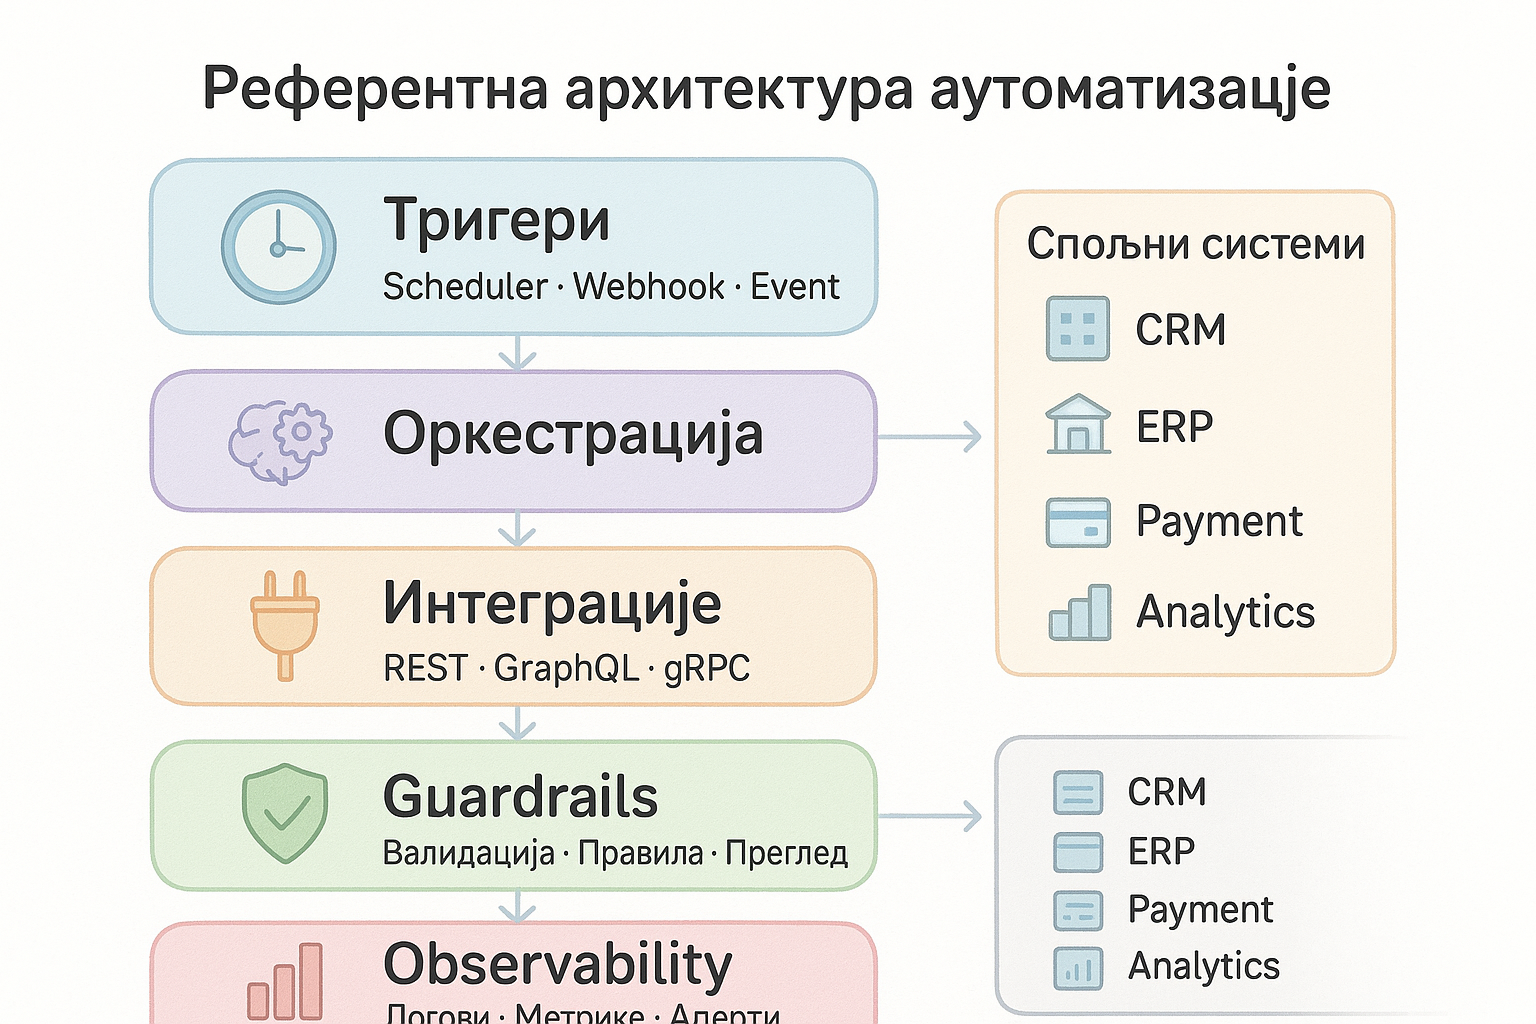
\includegraphics[width=0.95\textwidth]{slike/04/workflow_arcitekture.png}
    \caption{Референтна архитектура аутоматизације: слојеви и ток информација}
    \label{fig:04-6}
\end{figure}

\newpage

% =================================================================================
% POGLAVLJE 3
% =================================================================================

\section{Таксономија и Архитектура AI Система}
\label{sec:taksonomija-ai}

Развој савремених AI система захтева много више од избора „правог“ великог језичког модела (LLM).
Кључ успешне имплементације не лежи у самом моделу, већ у разумевању степена аутономије који систем треба да поседује и у архитектури која тај степен аутономије омогућава на контролисан и безбедан начин.
У пракси, један од најчешћих проблема у комуникацији између инжењера, менаџмента и клијената јесте
терминолошка конфузија. Појмови попут \textit{chatbota}, \textit{RAG sistema} и \textit{AI agenata} често се користе као синоними, иако представљају фундаментално различите архитектурне приступе.
Последица тога су нереална очекивања (нпр. да chatbot „сам нешто уради“) или, са друге стране,
прекомерно сложена решења за једноставне проблеме.

Ово поглавље уводи таксономију AI система засновану на нивоу аутономије и одговорности система.
Уместо да се AI посматра као монолитна технологија, системи се класификују дуж континуума:
од пасивних, реактивних модела који само генеришу текст, до комплексних, вишекомпонентних система
способних за планирање, извршавање акција и сарадњу са другим агентима.

Посебан фокус стављен је на разлику између:
\begin{itemize}
    \item Генеративних способности - шта систем може да напише,
    \item Оперативних способности - шта систем може да уради,
    \item Степена одговорности - који систем преузима у реалном окружењу.
\end{itemize}
\noindent
Како се крећемо ка вишим нивоима аутономије, AI системи престају да буду само алати за подршку кориснику,
а постају активни учесници у пословним и техничким процесима.
Са тим растом моћи пропорционално расте и потреба за јасном архитектуром, контролом тока извршења,
управљањем стањем, као и механизмима за опоравак од грешака.

Структура поглавља прати ову прогресију и уводи четири јасно раздвојена нивоа:
\begin{enumerate}
    \item AI асистенте у потпуности ослоњени ка LLM закључивање,
    \item RAG системе који додају утемељење у реалним подацима,
    \item Аутономне агенте способне за доношење одлука и извршавање акција,
    \item Мулти-агентске системе који омогућавају оркестрацију и колективно решавање сложених проблема.
\end{enumerate}
\noindent
Циљ овог поглавља није да промовише „најнапреднији“ приступ, већ да пружи инжењерски оквир за доношење
исправне одлуке: \textit{који ниво архитектуре је довољан, а који је непотребно сложен за конкретан проблем}.


\subsubsection*{Ниво 1: AI Асистенти (LLM закључивање)}

AI Асистенти представљају најосновнији и најраширенији облик примене генеративне вештачке интелигенције.
Они су примарно дизајнирани као интерфејси за закључивање над великим језичким моделима (LLM),
без трајног памћења, без аутономије и без директног утицаја на спољашње системе.
У архитектонском смислу, AI асистент је типично стателесс сервис:
сваки кориснички упит се обрађује независно, а сав „контекст“ који модел користи мора бити експлицитно
прослеђен унутар самог захтева (промпт-а).
Модел не поседује сопствено стање које се одржава између сесија, нити разуме континуитет интеракције
изван онога што му је тренутно дато као улаз.
Због тога се овај ниво често описује као примена LLM-а над текстом, приликом чега се
изводи пробабилистичко закључивање и враћа генерисани текст као одговор.
Примери таквих система су општи AI асистенти базирани на моделима попут GPT-4.1, Claude 4.5 или Qwen 3,
када се користе без додатне инфраструктуре (меморије, алата или екстерних извора података).

Иако је кориснички доживљај често антропоморфан (модел делује као да „разуме“, „зна“ или „размишља“),
унутрашњи механизам рада је знатно једноставнији, али математички софистициран~\cite{bender2021}.
AI асистенти функционишу на принципу предикције наредног токена (енг. \textit{Next Token Prediction})~\cite{vaswani2017,brown2020}.
За дати низ претходних токена (речи, делова речи или симбола), модел рачуна вероватноће могућих наредних
токена и бира следећи токен на основу тих вероватноћа.
Овај процес се понавља итеративно док се не генерише комплетан одговор.

Кључно је нагласити да модел:
\begin{itemize}
    \item не поседује унутрашњи појам истинитости или лажности,
    \item не проверава чињенице у реалном времену,
    \item не разликује „знање“, „претпоставку“ и „измишљање“ на концептуалном нивоу.
\end{itemize}
\noindent
За модел, тврдње попут „Париз је главни град Француске“ и „Париз је главни град Немачке“ нису
логички објекти са вредношћу истине, већ секвенце токена са различитим вероватноћама појављивања
у сличним контекстима током тренинга.

Овакав начин рада намеће неколико фундаменталних ограничења која су заједничка свим AI асистентима
на овом нивоу аутономије.

\begin{itemize}
    \item \textbf{Замрзнуто знање (Static Knowledge):}
    LLM модели не „уче“ након завршетка тренинга.
    Њихово знање је временски ограничено тренутком пресека података коришћених за тренирање.
    Догађаји, промене прописа, цене, или интерни документи који су настали након тог тренутка
    за модел не постоје, осим ако нису експлицитно унети у промпт.

    \item \textbf{Халуцинације:}
    Када модел нема довољно информација да поуздано одговори, он не сигнализира незнање
    на људски начин, већ наставља процес генерисања текста~\cite{ji2023hallucination}.
    Резултат су одговори који су лингвистички уверљиви, граматички исправни и често стилистички
    ауторитативни, али чињенично нетачни.
    Ово понашање није грешка у имплементацији, већ директна последица пробабилистичке природе модела.

    \item \textbf{Изолованост (Sandbox):}  
    Стандардни AI асистент нема приступ спољашњем свету.
    Он не види базе података, не приступа интернету, не може да провери стање система нити да
    изврши акцију.
    Све информације којима располаже морају бити садржане у самом упиту или већ присутне у
    параметрима модела из тренинга.
\end{itemize}
\noindent
Ова ограничења чине AI асистенте пасивним системима:
они реагују на кориснички унос, али не иницирају активности, не доносе одлуке које имају последице
у реалном окружењу и не сносе оперативну одговорност.

Упркос наведеним ограничењима, AI асистенти су изузетно корисни када се користе у правом контексту.
Њихова снага лежи у раду са текстом и симболима, а не у интеракцији са реалним системима.

Типичне и оправдане примене овог нивоа укључују:
\begin{itemize}
    \item креативно и техничко писање,
    \item сумирање и реструктурирање текста који корисник обезбеди,
    \item превођење између природних језика,
    \item помоћ при програмирању (code suggestions, објашњења, рефакторисање),
    \item генерисање идеја, нацрта и концептуалних објашњења.
\end{itemize}
\noindent
AI асистент не гарантује тачност, не проверава изворе и не извршава акције, он пружа језичку и когнитивну подршку, али не преузима улогу аутономног система. Пример AI асистента у \textit{n8n} дат је на слици~\ref{fig:04-7}.

\begin{figure}[h!]
    \centering
    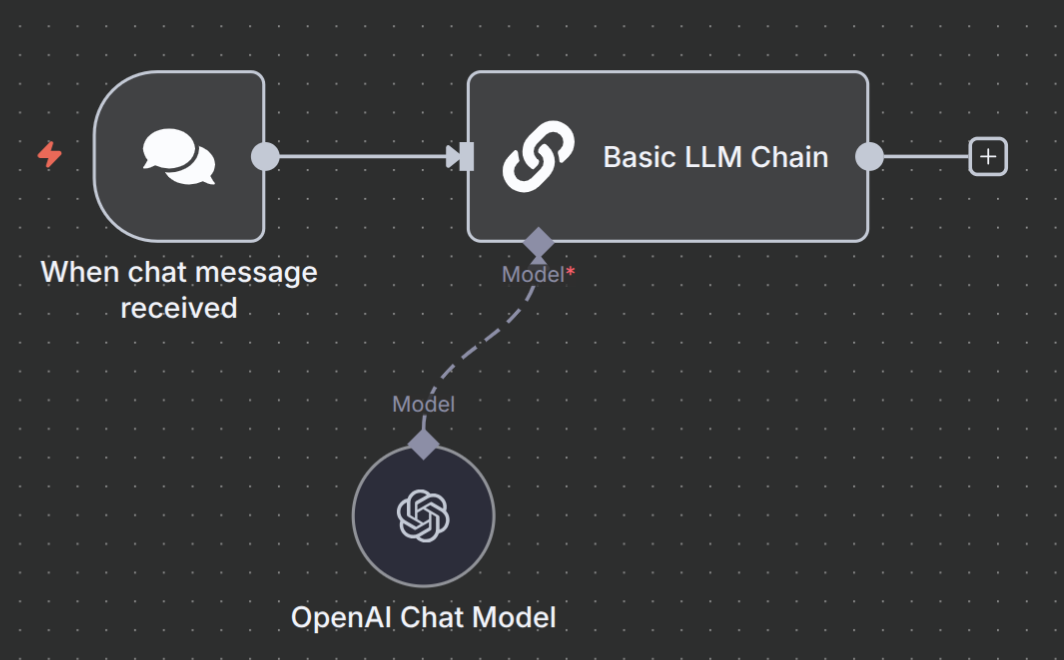
\includegraphics[width=0.8\textwidth]{slike/04/Base LLM.png}
    \caption{AI асистент у \textit{n8n}}
    \label{fig:04-7}
\end{figure}


\subsubsection*{Ниво 2: RAG Системи (Retrieval-Augmented Generation)}

Једно од кључних ограничења великих језичких модела (LLM) јесте чињеница да је њихово знање
замрзнуто у тренутку тренирања и да не обухвата специфичне, интерне или ажуриране информације
организације у којој се користе. Поред тога, LLM модели су склони тзв. халуцинацијама – генерисању
уверених, али нетачних одговора када немају довољно поуздан контекст.
Како би се ови проблеми превазишли, развијена је архитектура RAG (енг. \textit{Retrieval-Augmented Generation})~\cite{lewis2020rag,gao2024ragsurvey},
која комбинује предности класичних система за претрагу информација и генеративних AI модела.
Уместо да се LLM посматра као свеобухватна „енциклопедија“, RAG га трансформише у
процесор информација који активно користи спољне изворе знања у реалном времену.
У овом приступу, модел више не одговара искључиво на основу параметара научених током тренирања,
већ генерише одговор на основу \textit{relevantnog konteksta} који му се динамички доставља
из интерне базе знања организације.
RAG системи се фундаментално разликују од класичних претраживача заснованих на кључним речима
(\textit{keyword search}). Уместо тражења дословног поклапања термина,
RAG користи семантичку претрагу, која се заснива на значењу текста, а не на његовој форми.
На тај начин, систем може пронаћи релевантне информације чак и када се формулација питања
разликује од формулације у документима. Пример RAG система дат је на слици~\ref{fig:04-8}

\begin{figure}[h!]
    \centering
    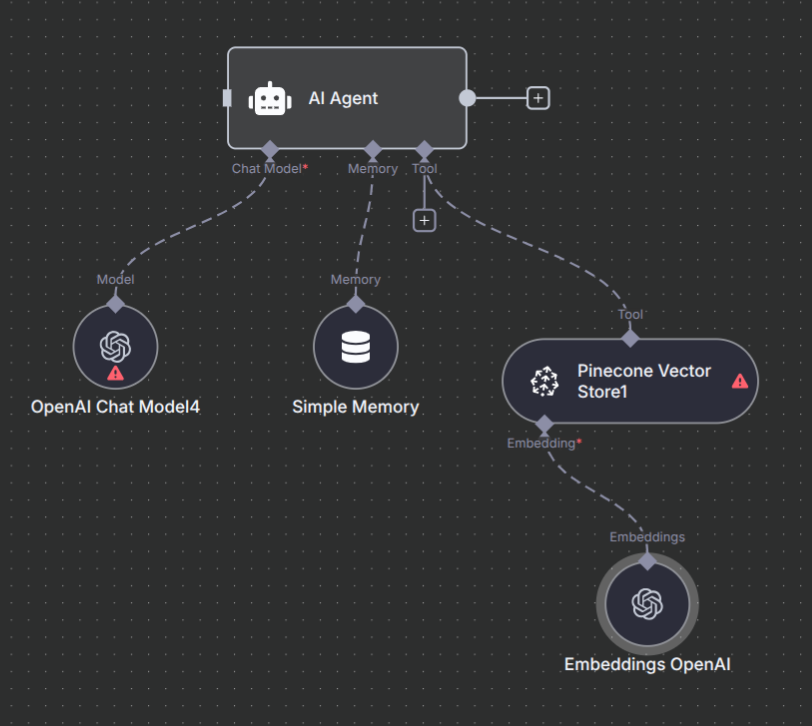
\includegraphics[width=0.7\textwidth]{slike/04/RAG.png}
    \caption{RAG у \textit{n8n}}
    \label{fig:04-8}
\end{figure}

Техничка архитектура RAG-а састоји се од неколико јасно раздвојених фаза:

\begin{enumerate}
    \item \textbf{Ingestion (Унос и припрема података):} \\
    Документи организације (PDF, Word, HTML, базе знања, вики странице) пролазе кроз процес обраде
    током којег се чисте, нормализују и деле на мање, логички смислене целине
    (енг. \textit{chunks}). Ова подела је кључна, јер превелики делови умањују прецизност претраге,
    док превише мали делови губе контекст.

    \item \textbf{Embedding (Векторизација значења):} \\
    Сваки сегмент текста се трансформише у нумеричку репрезентацију – вектор –
    коришћењем embedding модела~\cite{mikolov2013,reimers2019sbert}. Овај вектор кодира семантичко значење текста,
    тако да слични појмови и реченице имају сличне векторске репрезентације.
    Добијени вектори се складиште у специјализованој векторској бази података
    (нпр. Pinecone, Qdrant, Weaviate), оптимизованој за брзу семантичку претрагу~\cite{johnson2019faiss}.

    \item \textbf{Retrieval (Семантичка претрага):} \\
    Када корисник постави питање, и оно се преводи у векторски облик користећи исти embedding модел.
    Систем затим проналази оне сегменте из базе чији су вектори математички
    „најближи“ вектору питања, најчешће коришћењем косинусне сличности или сличних метрика~\cite{karpukhin2020dpr}.
    Резултат ове фазе није један документ, већ скуп најрелевантнијих контекстуалних исечака.

    \item \textbf{Synthesis (Контекстуална синтеза и генерисање):} \\
    Пронађени текстуални сегменти се затим комбинују са оригиналним корисничким питањем
    и прослеђују LLM моделу као додатни контекст у промпту.
    На основу тог контекста, модел генерише одговор који је директно утемељен
    у доступним документима, уместо у општем, генеричком знању.
\end{enumerate}

\begin{tcolorbox}[colback=yellow!10!white,colframe=orange!75!black,title=Prednost RAG-a: Utemeljenje (Grounding)]
Кључна предност RAG архитектуре јесте утемељење одговора у проверљивим изворима.
Уместо генеричких или спекулативних одговора, систем може експлицитно да се позове
на конкретан документ или део интерне документације, на пример:
\textit{„Према интерном правилнику, поглавље 3.2, процедура је следећа...“}.
У ситуацијама када релевантна информација не постоји у бази знања,
добро дизајниран RAG систем преферира одговор типа \textit{„Ta informacija nije dostupna“},
чиме се значајно смањује ризик од халуцинација и погрешних пословних одлука.


\end{tcolorbox}

\subsubsection*{Ниво 3: AI Агенти (Аутономни Системи)}

Док RAG архитектура проширује способности великих језичких модела додавањем
приступа екстерним изворима знања (метафорички, даје им „очи“),
AI агенти представљају следећи еволутивни корак: они систему додају „руке“,
односно способност да активно делује у окружењу.
Увођење агената означава прелаз са пасивних система, који искључиво генеришу
текстуалне одговоре, на аутономне системе за решавање проблема.
Такви системи не само да разумеју захтев корисника,
већ су у стању да самостално планирају, извршавају и прилагођавају низ акција
како би задати циљ био постигнут.

У контексту вештачке интелигенције, појам примене агената (енг. \textit{agency})
односи се на способност система да:
\begin{itemize}
    \item самостално интерпретира циљ,
    \item доноси одлуке о наредним корацима,
    \item извршава акције у окружењу,
    \item прилагођава понашање на основу повратних информација.
\end{itemize}

AI агент се, стога, дефинише као софтверски ентитет који аутономно
формира секвенцу акција неопходних за постизање задатог циља,
без потребе да сваки појединачни корак буде унапред експлицитно дефинисан од стране инжењера.
Ово представља кључну разлику у односу на традиционалну аутоматизацију.
Код класичних workflow система, сваки корак је унапред „закуцан“ у логику процеса.
Код агената, инжењер дефинише \textbf{шта} је циљ,
док агент самостално одлучује \textbf{како} ће до тог циља доћи.

Доминантна парадигма за имплементацију савремених AI агената данас је образац
\textbf{ReAct} (енг. \textit{Reasoning + Acting})~\cite{yao2022react,wang2024agents}.
Овај образац уводи цикличну структуру размишљања и деловања,
чиме се превазилази ограничење линеарних токова обраде.
Уместо да генерише комплетан одговор „у једном пролазу“,
агент функционише као систем са повратном спрегом,
континуирано прилагођавајући своје понашање на основу резултата претходних акција.

ReAct петља се састоји од три основне фазе:

\begin{enumerate}
    \item \textbf{Thought (Размишљање):} \\
    Агент анализира тренутно стање система, интерпретира кориснички захтев
    и доноси одлуку о следећем кораку.
    Овај корак представља интерни процес резоновања и планирања.

    \item \textbf{Action (Акција):} \\
    На основу донете одлуке, агент бира одговарајући алат
    (API позив, функцију, базу података, спољашњи сервис)
    и генерише конкретне параметре за његово извршавање.

    \item \textbf{Observation (Опсервација):} \\
    Резултат извршене акције се враћа агенту као нова информација.
    Овај резултат може бити податак, порука о успеху или грешка,
    и директно утиче на следећи циклус размишљања.
\end{enumerate}

Ова итеративна структура омогућава агенту да учи из сопствених акција
и динамички прилагођава стратегију извршавања. На овај начин агент у потпуности опонаша начине на који људи делују током решавања било ког проблема генерално.

\paragraph*{Пример извршења ReAct петље}

Размотримо кориснички захтев:
\textit{„Провери цену акција компаније Apple, конвертуј то у евре и пошаљи ми на Slack.“}

\begin{tcolorbox}[colback=white,colframe=black,title=Unutrašnji proces agenta]
\textbf{Итерација 1:}
\begin{itemize}
    \item \textit{Thought:} Потребна ми је тренутна цена акција Apple-а (AAPL).
    Тај податак није део мог статичког знања.
    \item \textit{Action:} \texttt{get\_stock\_price(symbol="AAPL")}
    \item \textit{Observation:} 185.50 USD
\end{itemize}

\textbf{Итерација 2:}
\begin{itemize}
    \item \textit{Thought:} Цена је у доларима, али корисник жели износ у еврима.
    \item \textit{Action:} \texttt{currency\_converter(from="USD", to="EUR", amount=185.50)}
    \item \textit{Observation:} 170.25 EUR
\end{itemize}

\textbf{Итерација 3:}
\begin{itemize}
    \item \textit{Thought:} Имам коначан резултат, потребно је обавестити корисника.
    \item \textit{Action:} \texttt{send\_slack\_message(channel="general", text="Cena AAPL je 170.25 EUR")}
    \item \textit{Observation:} Success: Message sent.
\end{itemize}

\textbf{Final Answer:} Задатак је успешно обављен.
\end{tcolorbox}
\noindent
Овај пример илуструје способност агента да повезује излаз једне акције
са улазом следеће (\textit{chaining}),
што је фундаментално различито од понашања класичних chatbot система.

\paragraph*{Техничка реализација: Tool Calling (Function Calling)}

Важно је нагласити да LLM модели сами по себи немају могућност извршавања кода
или интеракције са спољним системима.
Они функционишу искључиво као напредни процесори текста.
Да би агент могао да делује у реалном свету,
користи се механизам познат као \textit{Tool Calling} или \textit{Function Calling}~\cite{schick2023toolformer},
који омогућава да модел изабере одговарајући алат
и генерише структурирани захтев за његово извршење.

Доступни алати се агенту експлицитно описују приликом иницијализације,
најчешће кроз формалну спецификацију у облику \textbf{JSON Schema}~\cite{openai2024toolcalling,patil2023gorilla}.
Ова спецификација дефинише:
\begin{itemize}
    \item назив алата,
    \item опис његове намене,
    \item параметре које прихвата и њихове типове.
\end{itemize}

\begin{lstlisting}[language=json, caption={Definicija alata koju agent "vidi"}]
{
  "name": "get_weather",
  "description": "Dohvata trenutnu temperaturu za dati grad",
  "parameters": {
    "type": "object",
    "properties": {
      "city": {"type": "string", "description": "Ime grada"},
      "unit": {"type": "string", "enum": ["celsius", "fahrenheit"]}
    },
    "required": ["city"]
  }
}
\end{lstlisting}

На основу корисничког захтева,
модел не генерише слободан текстуални одговор,
већ структурирани позив алата са одговарајућим аргументима.
Рунтиме окружење затим извршава стварну функцију
и враћа резултат моделу као нови улаз за даљу обраду.

\paragraph*{Меморија и планирање}

Да би AI агент био заиста аутономан и способан за дуготрајно, смислено деловање,
мора поседовати механизме за памћење стања и планирање акција.
Без ових компоненти, систем се своди на простог извршиоца појединачних API позива,
без разумевања контекста, континуитета и циљне структуре задатка.
Меморија омогућава агенту да задржи информације о претходним корацима,
док планирање омогућава да те информације користи за доношење одлука
које нису локално оптималне, већ су усмерене ка остваривању крајњег циља.

Меморија агента не представља само историју порука,
већ структурисано управљање стањем система.
У пракси се разликују најмање два нивоа меморије:

\begin{itemize}
    \item \textbf{Краткорочна меморија (радна меморија):} \\
    Овај тип меморије обухвата контекст тренутне сесије и
    укључује резултате претходних акција, привремене варијабле,
    међурезултате и одлуке донете у току извршавања задатка. Величину и расположивост овог контекста директно ограничава \textit{context window} модела, при чему пракса показује да модели често „губе“ информације смештене у средини дугачких улаза~\cite{liu2023lostmiddle}.
    Краткорочна меморија се обично чува у оквиру рунтиме окружења
    (нпр. у меморији процеса или у оквиру контекста workflow-а)
    и брише се по завршетку задатка.

    \item \textbf{Дугорочна меморија (трајна меморија):} \\
    Дугорочна меморија омогућава агенту да задржи знање између различитих сесија
    и интеракција. Она се најчешће имплементира коришћењем
    векторских база података, које омогућавају семантичко складиштење
    и претрагу информација. На овај начин, агент може „памтити“:
    \begin{itemize}
        \item преференце и навике корисника,
        \item претходно решене проблеме и њихове исходе,
        \item интерне процедуре, документацију и правила,
        \item сопствена искуства из ранијих извршавања.
    \end{itemize}
\end{itemize}
\noindent
Важно је нагласити да дугорочна меморија не функционише као класична база чињеница,
већ као асоцијативни систем заснован на значењу, што омогућава флексибилно
призивање релевантних информација у различитим контекстима.

Поред меморије, кључна компонента аутономије јесте способност планирања.
Уместо да реагује искључиво на наредни корак,
агент је у стању да сагледа циљ у целини
и разложи га на низ међусобно зависних под-задатака.

За ову сврху се користе технике резоновања попут:
\begin{itemize}
    \item \textit{Chain of Thought} – експлицитно размишљање кроз кораке~\cite{wei2022cot},
    \item \textit{Self-Consistency} – узорковање више путања и избор најконзистентнијег закључка~\cite{wang2022selfconsistency},
    \item \textit{Tree of Thoughts} – гранање и евалуација више путања резоновања~\cite{yao2023tot},
    \item хијерархијско планирање – разлагање циља на фазе и активности,
    \item итеративно репланирање – прилагођавање плана током извршавања~\cite{shinn2023reflexion,madaan2023selfrefine}.
\end{itemize}

На пример, за задатак \textit{„Направи анализу тржишта“},
агент може прво формирати апстрактан план
(прикупљање података, анализа, синтеза),
а затим сваку фазу додатно разложити на конкретне акције
(претрага извора, екстракција података, поређење цена, генерисање извештаја).

\paragraph*{Само-корекција и учење из грешака}

Једна од најважнијих особина аутономних агената јесте способност
\textbf{само-корекције}.
У овом моделу, грешке се не посматрају као фатални проблеми,
већ као нова информација у процесу резоновања.

Ако нека акција не успе (нпр. API врати грешку, ресурс није доступан,
или резултат не задовољава очекивања),
агент ту информацију прима кроз фазу опсервације
и користи је за прилагођавање наредних корака.
То може укључивати промену алата, модификацију параметара
или редефинисање плана.

Ова отпорност на грешке (\textit{resilience})
омогућава агентима да функционишу у реалним,
динамичким и непредвидивим окружењима,
где потпуна контрола над спољним системима није могућа.
Пример једноставног AI система  за слање мотивационих порука дат је на слици~\ref{fig:04-9}. LLM се користи искључиво за генерисање текста, док су извори података и акције слања
реализовани кроз детерминистичке n8n чворове.

\begin{figure}[h!]
    \centering
    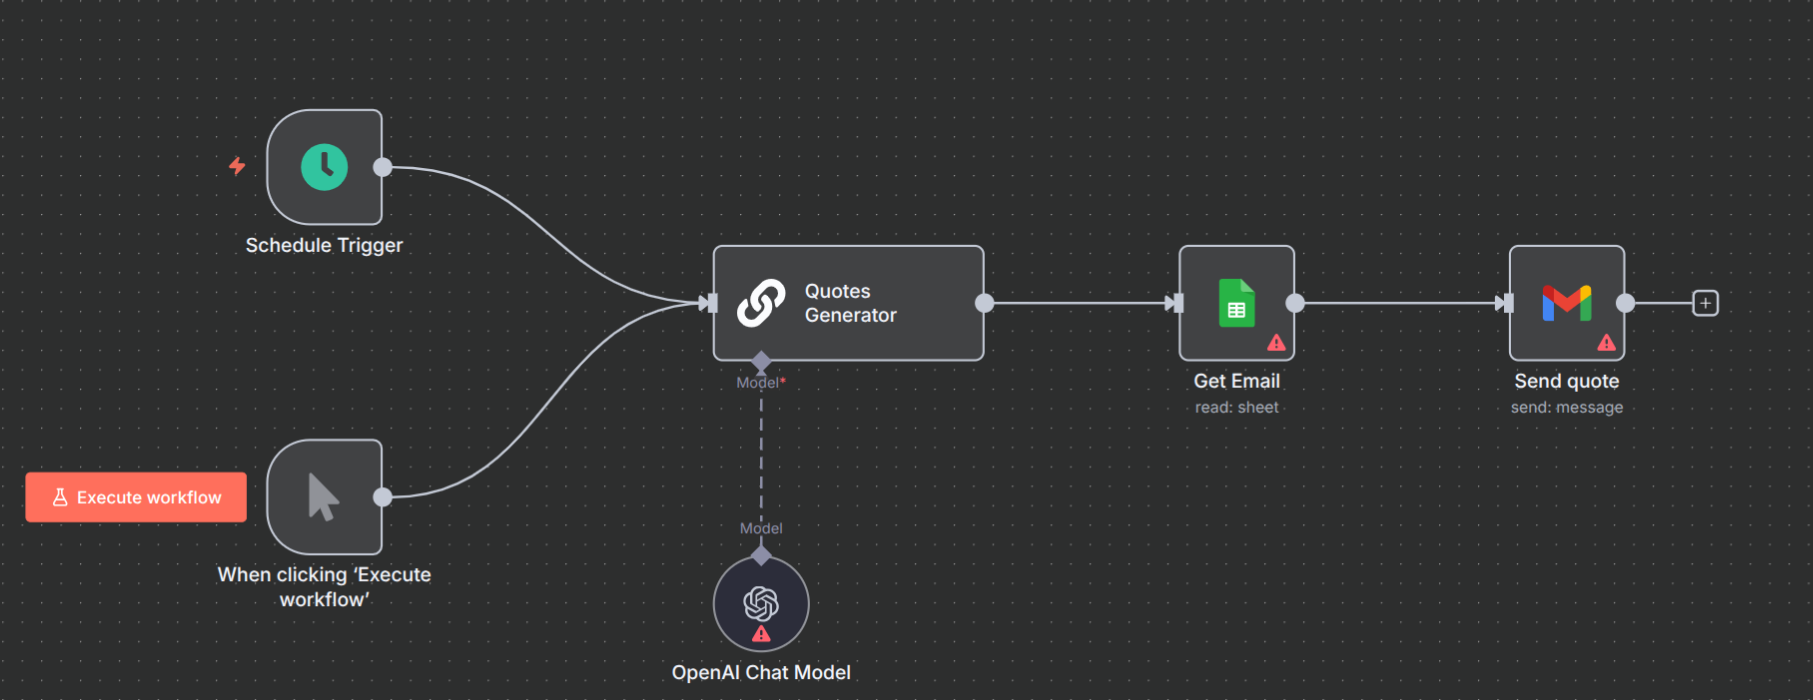
\includegraphics[width=0.85\textwidth]{slike/04/primer_agenta_quote.png}
    \caption{Агент за генерисање мотивационих порука у \textit{n8n}}
    \label{fig:04-9}
\end{figure}

% =================================================================================
% POGLAVLJE 3.4 - PROŠIRENA VERZIJA
% =================================================================================

\subsection{Ниво 4: Мулти-Агентски Системи (MAS)}

Док појединачни агенти представљају моћне алате, они поседују инхерентна ограничења када се суоче са задацима високе комплексности.
Један агент опремљен са десет различитих алата и дугачким системским промптом често постаје "збуњен" – губи фокус, халуцинира инструкције или неисправно бира алате. Ово је познато као проблем "уског грла контекста" (енг. \textit{Context Bottleneck}).
Решење лежи у Мулти-Агентским Системима (MAS)~\cite{wu2023autogen,park2023agents,li2023camel}. Ови системи симулирају организациону структуру људских тимова, где се комплексан проблем разбија на мање целине које решавају специјализовани, колаборативни агенти.

Кључна предност MAS архитектуре је модуларност. Уместо једног генералног агента ("Jack of all trades"), креира се тим експерата:
\begin{itemize}
    \item Сваки агент има свој, високо специфичан системски промпт (нпр. "Ти си сениор Python инжењер...").
    \item Сваки агент има приступ само оним алатима који су му неопходни (смањује ризик од грешке).
    \item Агенти могу користити различите LLM моделе (нпр. јефтинији модел за сумирање, скупљи и паметнији модел за решавање логике).
\end{itemize}

У зависности од природе проблема, инжењери бирају различите топологије сарадње између агената. Три најдоминантнија обрасца су:

\paragraph*{1. Хијерархијска сарадња (Supervisor / Router Pattern)}
Овај образац имитира корпоративну структуру "Менаџер - Запослени".

\begin{itemize}
    \item \textbf{Супервизор (Router):} Централни чвор система. Овај агент обично користи напредан модел (нпр. GPT-4o). Он не извршава задатке директно. Његова улога је да анализира захтев корисника, разбије га на под-задатке и одлучи којем раднику да делегира посао. Такође, он врши инспекцију резултата пре него што их врати кориснику.
    \item \textbf{Радници (Workers):} Специјализовани агенти који оперишу у изолацији.
\end{itemize}

\textbf{Пример тока података:}
\begin{enumerate}
    \item Корисник: „Напиши ми код за Snake игрицу у Python-у и генериши слику за лого.“
    \item Супервизор анализира и каже: „За кодирање зовем \textit{DevAgent}, за лого зовем \textit{DesignAgent}.“
    \item \textit{DevAgent} пише код и враћа га Супервизору.
    \item \textit{DesignAgent} црта слику и враћа је Супервизору.
    \item Супервизор спаја оба резултата и шаље финални одговор кориснику.
\end{enumerate}

\paragraph*{2. Секвенцијална сарадња (енг. \textit{The Assembly Line)}}
Овај образац функционише као производна трака. Излаз једног агента постаје директан улаз за следећег агента. Овде не постоји централни менаџер који одлучује – путања је унапред дефинисана (\textit{Hard-coded workflow}).

Ово је идеално за процесе који имају стриктан редослед.

\textbf{Пример: Креирање Блога}
\begin{itemize}
    \item \textbf{Агент 1 (Истраживач):} Претражује Google на задату тему и креира сирови сажетак чињеница. $\rightarrow$ Прослеђује текст.
    \item \textbf{Агент 2 (Писац):} Узима чињенице и пише ангажован чланак пратећи SEO правила. $\rightarrow$ Прослеђује нацрт.
    \item \textbf{Агент 3 (Уредник):} Чита нацрт, исправља граматичке грешке и проверава тон комуникације. $\rightarrow$ Финални текст.
\end{itemize}

Предност овог приступа је предвидљивост и лакоћа дебаговања, јер је сваки корак јасно раздвојен.

\paragraph*{3. Колаборативна дебата (енг. \textit{Joint Collaboration / Network)}}
Ово је најкомплекснији, али и најмоћнији облик сарадње, инспирисан академским или инжењерским "brainstorming" сесијама. Агенти нису пасивни извршиоци, већ активно комуницирају једни са другима у петљи, критикују туђи рад и предлажу побољшања.

У овом моделу често се уводи улога Критичара (Critique Agent).

\textbf{Пример: Развој Софтвера}
\begin{itemize}
    \item \textbf{Coder Agent:} Пише иницијалну верзију кода~\cite{chen2021codex}.
    \item \textbf{Reviewer Agent:} Анализира тај код. Не извршава га, већ тражи сигурносне пропусте (бугове). Враћа feedback: "Линија 42 је несигурна, може доћи до SQL Injection напада."
    \item \textbf{Coder Agent:} Прима критику, размишља („Thought: У праву је, морам да санитизујем input“) и пише верзију 2.0.
    \item Процес се понавља док Reviewer Agent не каже "Одобрено"~\cite{wang2023voyager}.
\end{itemize}
\noindent
Овај итеративни процес доказано повећава квалитет излазног резултата у односу на "Single-shot" генерисање (где модел има само једну шансу да погоди решење).

\paragraph*{Управљање стањем (Shared State)}

Једно од најважнијих техничких питања у дизајну мулти-агентских система јесте:
\textit{Како агенти деле информације и како се обезбеђује конзистентност њиховог рада?}
За разлику од single-agent система, где је ток размишљања и акција садржан у једној инстанци,
мулти-агентски системи захтевају експлицитан механизам за размену контекста.
Без јасно дефинисаног заједничког стања, агенти би радили изоловано, што би довело до
дуплирања рада, контрадикторних одлука или губитка информација.

У савременим оквирима за изградњу MAS-а (као што су LangGraph или AutoGen),
овај проблем се решава увођењем концепта \textbf{Дељеног Стања} (\textit{Shared State} или \textit{Graph State}).
Дељено стање представља централни, структурирани објекат који садржи све релевантне информације
о тренутном статусу задатка и који се прослеђује између агената током извршавања система.

Технички, дељено стање је најчешће имплементирано као JSON објекат који обухвата:
\begin{itemize}
    \item оригинални захтев корисника,
    \item парцијалне резултате рада појединачних агената,
    \item мета-информације о томе који кораци су завршени,
    \item повратне информације (feedback) и одлуке надређених агената,
    \item сигнализацију да ли је задатак завршен или захтева додатну обраду.
\end{itemize}

\begin{lstlisting}[language=json, caption={Primer deljenog stanja u multi-agentskom sistemu}]
{
  "user_request": "Napravi izveštaj o prodaji",
  "data_gathered": true,
  "raw_data": [ ... ],
  "draft_report": "Prodaja je porasla za 20%...",
  "manager_approval": false,
  "feedback": "Dodaj grafikone u sekciju 3"
}
\end{lstlisting}

Сваки агент у систему добија приступ овом стању као улаз.
На основу свог системског промпта и улоге, агент:
\begin{enumerate}
    \item чита релевантне делове стања,
    \item извршава своју специфичну одговорност,
    \item ажурира стање новим информацијама или одлукама,
    \item прослеђује ажурирано стање следећем агенту или назад супервизору.
\end{enumerate}

На пример, аналитички агент може да попуни поље \texttt{raw\_data},
писац извештаја генерише \texttt{draft\_report},
док супервизорски агент мења вредност \texttt{manager\_approval} у \texttt{true}
када процени да је резултат прихватљив.

Овакав приступ има неколико кључних предности:
\begin{itemize}
    \item омогућава \textbf{транспарентност} процеса — јасно је у којој фази се задатак налази,
    \item олакшава \textbf{debugging и аудит} јер се свака одлука рефлектује у стању,
    \item омогућава \textbf{паралелни рад} агената над различитим деловима истог проблема,
    \item спречава неконтролисано „размишљање“ модела ван дефинисаног контекста.
\end{itemize}

Истовремено, дељено стање намеће и строгу дисциплину у дизајну система:
што је стање комплексније и неструктурисаније, већи је ризик од грешака,
неконзистентности и неочекиваних понашања агената.
Због тога се у пракси често уводе формалне шеме (\textit{schemas}) и валидација стања,
како би се осигурало да сваки агент види и мења само оне делове стања за које је задужен. 

На слици~\ref{fig:04-10} дат је пример мулит-агентског система у \textit{n8n}. Улазни захтеви се нормализују и прослеђују супервизорском агенту, који на основу садржаја
делегира задатке специјализованим агентима (е-маил, истраживање, управљање задацима, календар).
Сваки агент користи велики језички модел искључиво за разумевање захтева, док се стварне
акције извршавају кроз детерминистичке API позиве.

\subsubsection{Компаративна анализа система}

Табела~\ref{tab:04-2} приказује компаративни преглед кључних функционалних способности четири доминантне категорије савремених AI система: класичних AI асистената заснованих на великим језичким моделима (LLM), RAG система (Retrieval-Augmented Generation), аутономних AI агената и мулти-агентских система (MAS).

\textbf{AI асистенти} представљају најосновнији облик интеракције са великим језичким моделима. Њихова функционалност се своди на генерисање одговора на основу корисничког упита, без експлицитне везе са спољним изворима знања или могућности извршавања акција. Овакви системи су у потпуности реактивни: не поседују сопствену иницијативу, не памте стање између интеракција и не могу доносити одлуке ван граница једног промпт–одговор циклуса. Због тога су погодни за опште информативне задатке, објашњења и креативно генерисање садржаја, али нису адекватни за комплексне пословне или оперативне процесе.

\textbf{RAG системи} представљају значајан корак напред у односу на чисте AI асистенте. Увођењем семантичке претраге над екстерним документима (путем embedding-а и векторских база), RAG омогућава утемељење генерисаних одговора у конкретним изворима знања. Ипак, иако RAG системи поседују дугорочну меморију у виду документационог репозиторијума, они су и даље фундаментално пасивни. Њихова улога је ограничена на побољшано одговарање на упите, без способности планирања, извршавања акција или управљања сложеним токовима рада.

\textbf{AI агенти} уводе концепт аутономије и оперативне интелигенције. За разлику од асистента и RAG система, агенти су дизајнирани да раде у итеративној петљи \textit{Thought–Action–Observation}, при чему могу самостално доносити одлуке, позивати спољне алате (API-је, базе података, скрипте), анализирати резултате и прилагођавати даље кораке. Кључна разлика је у томе што агент поседује унутрашње стање (сессион мемори), способност планирања и механизме само-корекције. Тиме агент прелази из пасивне у активну улогу, где може извршавати задатке од почетка до краја уз минималну људску интервенцију.

\textbf{Мулти-агентски системи (MAS)} представљају најнапреднији облик агентске архитектуре. Они су неопходни у сценаријима где задаци нису линеарни, већ захтевају паралелну обраду, специјализацију и координацију више аутономних ентитета. Уместо једног универзалног агента, MAS се састоји од више агената са јасно дефинисаним улогама (нпр. истраживач, планер, извршилац, евалуатор). Сваки агент је оптимизован за своју функцију путем посебног промпта, алата и ограничења, док централни оркестрациони механизам управља разменом информација и делегирањем задатака.

Кључна предност мулти-агентских система лежи у њиховој способности да решавају комплексне, нелинеарне проблеме на дистрибуиран начин. Паралелизација рада, хијерархијско планирање и међусобна евалуација агената доводе до веће робусности, тачности и скалабилности система. Због тога се MAS архитектуре све чешће примењују у напредним пословним аутоматизацијама, истраживачким платформама, аутономним аналитичким системима и сложеним организационим процесима.

Сумарно, табела~\ref{tab:04-2} јасно показује да разлика између наведених система није само у количини функционалности, већ у њиховој епистемолошкој и оперативној улози. Док AI асистенти и RAG системи служе као алати за подршку кориснику, AI агенти и посебно мулти-агентски системи представљају самосталне извршне ентитете, способне да преузму активну улогу у доношењу одлука и реализацији комплексних задатака.

\begin{small}
\begin{longtable}{|p{5.2cm}|c|c|c|c|}
\caption{Матрица способности: Chatbot vs RAG vs AI Агент vs Мулти-Агент систем}\label{tab:04-2}\\
\hline
\textbf{Способност / карактеристика}
& \textbf{AI Асистент (LLM)}
& \textbf{RAG}
& \textbf{AI Агент}
& \textbf{Мулти-Агент} \\
\hline
\endfirsthead
\hline
\textbf{Способност / карактеристика}
& \textbf{AI Асистент (LLM)}
& \textbf{RAG}
& \textbf{AI Агент}
& \textbf{Мулти-Агент} \\
\hline
\endhead
\hline
\endfoot

Одговарање на питања / генерисање текста & Х & Х & Х & Х \\
\hline
Утемељење у екстерним документима (grounding) &  & Х & Х & Х \\
\hline
Семантичка претрага (embedding + вектор база) &  & Х & Х & Х \\
\hline
Структурисан излаз (JSON схема / валидација) &  &  & Х & Х \\
\hline
Извршавање акција (tool/function calling) &  &  & Х & Х \\
\hline
Итеративна петља (ReAct: Thought--Action--Observation) &  &  & Х & Х \\
\hline
Краткорочна меморија стања (session state) &  &  & Х & Х \\
\hline
Дугорочна меморија између сесија (persistent memory) &  & Х & Х & Х \\
\hline
Планирање и декомпозиција задатака &  &  & Х & Х \\
\hline
Само-корекција и репланирање након грешке &  &  & Х & Х \\
\hline
Специјализација улога (нпр. Researcher, Executor, Critic) &  &  &  & Х \\
\hline
Делегирање и координација (task routing између агената) &  &  &  & Х \\
\hline
Паралелизација рада (истовремени суб-таскови) &  &  &  & Х \\
\hline
Централна контрола и guardrails на нивоу организације &  & Х & Х & Х \\
\hline
Observability: логови/метрике/tracing по корацима &  & Х & Х & Х \\
\hline
\end{longtable}
\end{small}


\begin{figure}[h!]
    \centering
    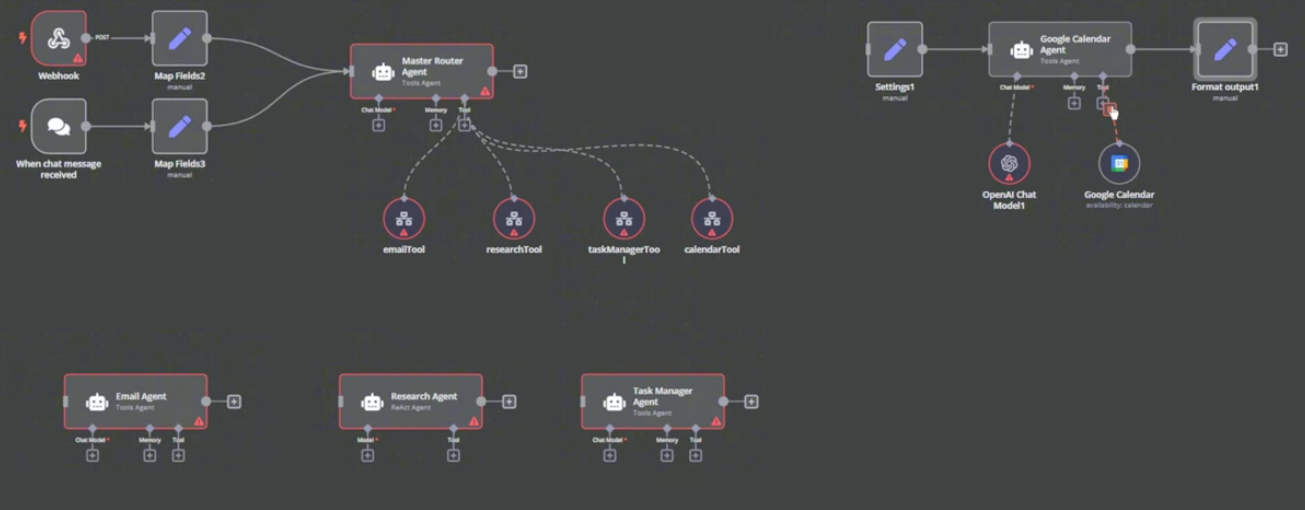
\includegraphics[width=0.95\textwidth]{slike/04/multiagent.png}
    \caption{Мултиагентски систем у \textit{n8n}}
    \label{fig:04-10}
\end{figure}


\newpage

% =================================================================================
% POGLAVLJE: VELIKI JEZIČKI MODELI (LLM)
% =================================================================================

% =================================================================================
% POGLAVLJE: VELIKI JEZIČKI MODELI - AKADEMSKA VERZIJA
% =================================================================================

\section{Велики Језички Модели: Когнитивни мотор система}

У основи савремених система за аутоматизацију, од једноставних процесора текста до комплексних мулти-агентских архитектура, налази се технологија великих језичких модела (енг. \textit{Large Language Models - LLM}).

За успешно пројектовање аутоматизованих система у алатима као што је \textit{n8n}, императив је превазићи површно разумевање LLM-а као „напредног chatbot-а“. Инжењерски приступ захтева дубинско познавање архитектуре, ограничења и пробабилистичке природе ових модела. Разумевање интерне логике модела омогућава предвиђање понашања система, оптимизацију потрошње ресурса (токена) и имплементацију механизама за контролу грешака.

\subsection{Дефиниција и декомпозиција појма LLM}

Велики језички модел се дефинише као напредни систем вештачке интелигенције, заснован на архитектури дубоких неуронских мрежа (примарно \textit{Transformer} архитектури)~\cite{vaswani2017,goodfellow2016}, који је способан да разуме, генерише и манипулише симболичким системима, укључујући природне језике и програмске кодове~\cite{devlin2019,brown2020}.

Водећи модели на тржишту, као што су GPT-4.1 (OpenAI)~\cite{openai2023gpt4,bubeck2023}, Claude 4.5 (Anthropic)~\cite{anthropic2024claude} и DeepSeek v3.2, представљају врхунац ове технологије. Отворена алтернатива, као што је LLaMA породица модела~\cite{touvron2023}, као и Mistral~\cite{jiang2023mistral}, BLOOM~\cite{bigscience2022bloom} и PaLM~\cite{chowdhery2022palm}, такође је допринела ширем екосистему истраживачких и комерцијалних модела. Да би се разумела њихова комплексност, неопходно је анализирати три компоненте њиховог назива:

\paragraph{Велики (Large)}
Атрибут "Велики" односи се на две кључне димензије скалабилности:
\begin{itemize}
    \item \textbf{Обим података за тренинг:} Ови модели се тренирају на корпусима података који се мере у петабајтима, обухватајући значајан део јавно доступног интернета (Common Crawl), милионе дигитализованих књига, научних радова и репозиторијума кода.
    \item \textbf{Број параметара:} Параметри представљају интерне променљиве (тежине веза у неуронској мрежи) које модел подешава током процеса учења. Савремени модели поседују од неколико милијарди (7Б) до преко билион (1Т+) параметара~\cite{kaplan2020scaling,fedus2022switch,hoffmann2022chinchilla}. Број параметара директно корелира са способношћу модела да апстрахује комплексне концепте и нијансе у расуђивању~\cite{wei2022emergent,hendrycks2021mmlu}.
\end{itemize}

\paragraph{Језички (Language)}
Иако се називају "језичким", ови модели суштински оперишу над симболима (реч, број, знак). У контексту LLM-а, језик се не односи само на лингвистичке системе (српски, енглески), већ на било који систем симбола са дефинисаном синтаксом и семантиком. То укључује програмске језике (Python, JavaScript), формате података (JSON, XML) и математичку нотацију. Модел учи мапирање и односе између ових симбола, што му омогућава "превођење" природног захтева у извршни код.

\paragraph{Модел (Модел)}
Ово је концептуално најважнија дистинкција. LLM није база података, нити енциклопедија. Он је \textbf{статистичка репрезентација} података на којима је трениран. Он не "складишти" информације у класичном смислу (као фајлове), већ моделује вероватноћу појављивања одређених секвенци симбола у одређеном контексту.

\subsection{Епистемолошка природа LLM-а: Компресија са губитком}

У популарним објашњењима, велики језички модели (LLM) се често описују као
„библиотека свих књига“ или „дигитални енциклопедијски ум“.
Иако је ова аналогија интуитивна, она је технички и епистемолошки непрецизна,
јер имплицира да модел поседује експлицитно складиштене чињенице и да
приликом одговарања врши процес \textit{претраге и проналажења} информација
(\textit{retrieval}).

Прецизнија инжењерска аналогија гласи:
\textbf{LLM представља екстремно компресовану репрезентацију великог дела јавно доступног
људског знања, изведену кроз процес компресије са губитком}
(\textit{lossy compression})~\cite{bender2021,zhao2023llmsurvey}.
Ова перспектива је кључна за разумевање како LLM модели „знају“,
али и зашто понекад греше на систематичан и предвидив начин.

Код класичних алгоритама за компресију података са губитком,
попут JPEG-а за слике или MP3-а за звук,
оригинални сигнал се не чува у потпуности.
Уместо тога, алгоритам идентификује статистичке обрасце
и уклања детаље који се сматрају мање важним за перцепцију.
На пример, JPEG алгоритам не памти вредност сваког појединачног пиксела,
већ апроксимира слику кроз фреквенцијске компоненте,
чувајући глобалне структуре, ивице и боје,
док се ситни детаљи жртвују ради смањења величине фајла.
Аналогно томе, LLM модели не памте појединачне реченице,
документе или чињенице из тренинг података.
Уместо тога, током тренирања они уче
статистичке обрасце у језику:
како се појмови повезују, које речи типично следе једна другу,
какве структуре имају објашњења, дефиниције и аргументи.
Резултат овог процеса није база знања,
већ параметарски модел (милијарде или трилиони тежина)
који представља компресовану мапу вероватноћа над језиком.

Много конфузије уноси чињеница да општа јавност најчешће поистовећује LLM са базом података, међутим разлика између истих је очигледна.
Ова разлика се може јасно илустровати поређењем класичних база података
и великих језичких модела:

\begin{itemize}
    \item \textbf{База података} функционише по принципу
    \textit{lookup} операције.
    Ако се затражи податак који постоји у бази,
    систем враћа тачно онај запис који је претходно уписан.
    Тачност је детерминистичка, а грешка углавном указује на
    непостојање или погрешан унос података.

    \item \textbf{LLM} функционише по принципу
    \textit{rekonstrukcije}.
    Када се моделу постави питање,
    он не претражује меморију у потрази за „тачним одговором“,
    већ генерише одговор токен по токен,
    на основу вероватноћа научених током тренирања.
    Другим речима, одговор се реконструише,
    а не проналази.
\end{itemize}
\noindent
Ова реконструктивна природа објашњава зашто LLM модели могу
давати изузетно флуентне и уверљиве одговоре чак и у ситуацијама
када немају експлицитно знање о траженој чињеници. 

\subsubsection*{Знање као дистрибуција, а не као чињеница}

Епистемолошки посматрано,
знање у LLM-у није скуп истинитих тврдњи,
већ \textbf{дистрибуција вероватноћа над могућим исказима}.
Модел „зна“ да су одређени одговори вероватнији од других
у датом контексту, али не поседује механизам
за проверу истинитости у реалном свету.

Због тога LLM може:
\begin{itemize}
    \item исправно објаснити општи концепт,
    \item погрешити у прецизном датуму, броју или цитату,
    \item самоуверено генерисати одговор и када информација не постоји.
\end{itemize}

Ово понашање није грешка у имплементацији,
већ директна последица начина на који је знање представљено у моделу.

\begin{tcolorbox}[colback=gray!10!white,colframe=black!75!white,title=Implikacija: Fenomen halucinacija]
Феномен тзв. \textbf{халуцинација} код LLM модела
није аномалија, већ очекивана последица реконструктивне природе система.
Када модел нема довољно информација или контекстуалних ограничења,
он и даље покушава да произведе највероватнији могући одговор,
што може резултирати текстом који је граматички исправан
и семантички уверљив, али фактички нетачан.

У инжењерској пракси, овај ризик се не решава
„бољим промптом“, већ архитектоним проширењима,
као што су RAG системи, валидација извора,
детерминистичка правила и људска верификација.
\end{tcolorbox}

\subsubsection*{Последице за дизајн AI система}

Разумевање LLM-а као система за компресију са губитком
има директне последице по дизајн поузданих AI решења.
LLM не треба користити као једини извор истине,
већ као компоненту за:
\begin{itemize}
    \item синтезу и објашњавање информација,
    \item генерисање текста и хипотеза,
    \item повезивање и интерпретацију постојећих података.
\end{itemize}
\noindent
За задатке који захтевају тачност, проверљивост и одговорност,
LLM мора бити интегрисан са екстерним изворима знања,
механизмима контроле и архитектурама попут RAG-а и AI агената~\cite{lin2022truthfulqa,liang2022helm}.


\subsection{Транзиција парадигме: Од детерминистичког ка стохастичком}

Имплементација LLM-а у пословне процесе означава фундаменталну промену у парадигми програмирања и аутоматизације.

\begin{enumerate}
    \item \textbf{Детерминистички системи (Традиционални софтвер):}
    Карактерише их предвидљивост. За исти улаз ($Input A$), софтвер ће увек, без изузетка, генерисати исти излаз ($Output B$). Логика је експлицитно кодирана ("иф-тхен-елсе").
    
    \item \textbf{Стохастички системи (LLM):}
    Карактерише их вероватноћа. За исти улаз, модел може генерисати различите варијације излаза, у зависности од параметара као што су \textit{Temperatura} и интерни сеед.
\end{enumerate}
\noindent
Улога инжењера аутоматизације се стога мења: уместо писања експлицитних инструкција за сваки могући сценарио, фокус се помера на управљање вероватноћом. Кроз технике промпт инжењеринга и валидацију структуре података (нпр. форсирање JSON излаза), циљ је ограничити стохастичку природу модела тако да он постане поуздан алат у пословном окружењу.


\subsection{Архитектура: Анатомија извршног окружења}

Са становишта софтверског инжењерства, Велики језички модел није магична црна кутија, већ јасно дефинисан софтверски артефакт. Да би се модел покренуо било да је реч о локалном покретању \textit{Qwen 3} модела на серверу компаније или коришћењу \textit{GPT-4.1} путем API-ја неопходно је присуство две фундаменталне компоненте. Раздвајање знања од логике извршавања је кључна карактеристика ове архитектуре.

Сваки LLM систем се састоји од:

\begin{enumerate}
    \item \textbf{Фајл са параметрима (Parameters File / The Weights):} \\
    Ово је статички бинарни фајл који представља замрзнуто знање модела.
    \begin{itemize}
        \item \textbf{Садржај:} Фајл не садржи речи, реченице или if-then правила. Он садржи милијарде (или билионе) бројева са покретним зарезом (\textit{floating-point numbers}), нпр. \texttt{0.00241, -0.5321}. Ови бројеви се називају \textbf{тежине (\textit{weights})} и организовани су у вишедимензионалне матрице познате као тензори.
        \item \textbf{Функција:} Тежине одређују јачину везе између вештачких неурона у мрежи. Оне су резултат процеса тренинга – математичке оптимизације која је трајала месецима. Фајл са параметрима је \textit{Read-Only} (само за читање) током коришћења модела; он се не мења док модел одговара на питања (осим у процесу финог подешавања).
        \item \textbf{Величина:} Величина овог фајла директно корелира са интелигенцијом модела. За модел од 70 милијарди параметара (70B), овај фајл може заузимати преко 140 GB простора на диску и захтева еквивалентну количину VRAM-а (видео меморије) да би се учитао.
    \end{itemize}

    \item \textbf{Извршни фајл (Run File / Inference Engine):} \\
    Ово је погон модела. То је релативно компактан програмски код (често написан у C++, Python-у или CUDA језику за графичке картице) који је одговоран за процес \textbf{инференције}.
    \begin{itemize}
        \item \textbf{Улога:} Овај код не поседује никакво знање. Његов задатак је чисто механички: он учитава гигантски фајл са параметрима у меморију и дефинише архитектуру (нпр. Transformer слојеве, Attention механизме).
        \item \textbf{Процес рада:} Када корисник пошаље текст, извршни фајл прво врши \textit{tokenizaciju} (претвара текст у низ бројева познатији под именом embedding). Затим спроводи те бројеве кроз математичке операције (матрично множење) користећи учитане тежине из фајла са параметрима. На крају, примењује функцију вероватноће (Softmax) да би израчунао који токен треба да буде следећи.
        \item \textbf{Универзалност:} Занимљиво је да исти извршни фајл може покретати различите мозгове (различите фајлове са параметрима), под условом да деле исту архитектуру.
    \end{itemize}
\end{enumerate}
\noindent
Сликовити приказ рада LLM система дат је на слици~\ref{fig:04-11}.


\begin{figure}[h!]
    \centering
    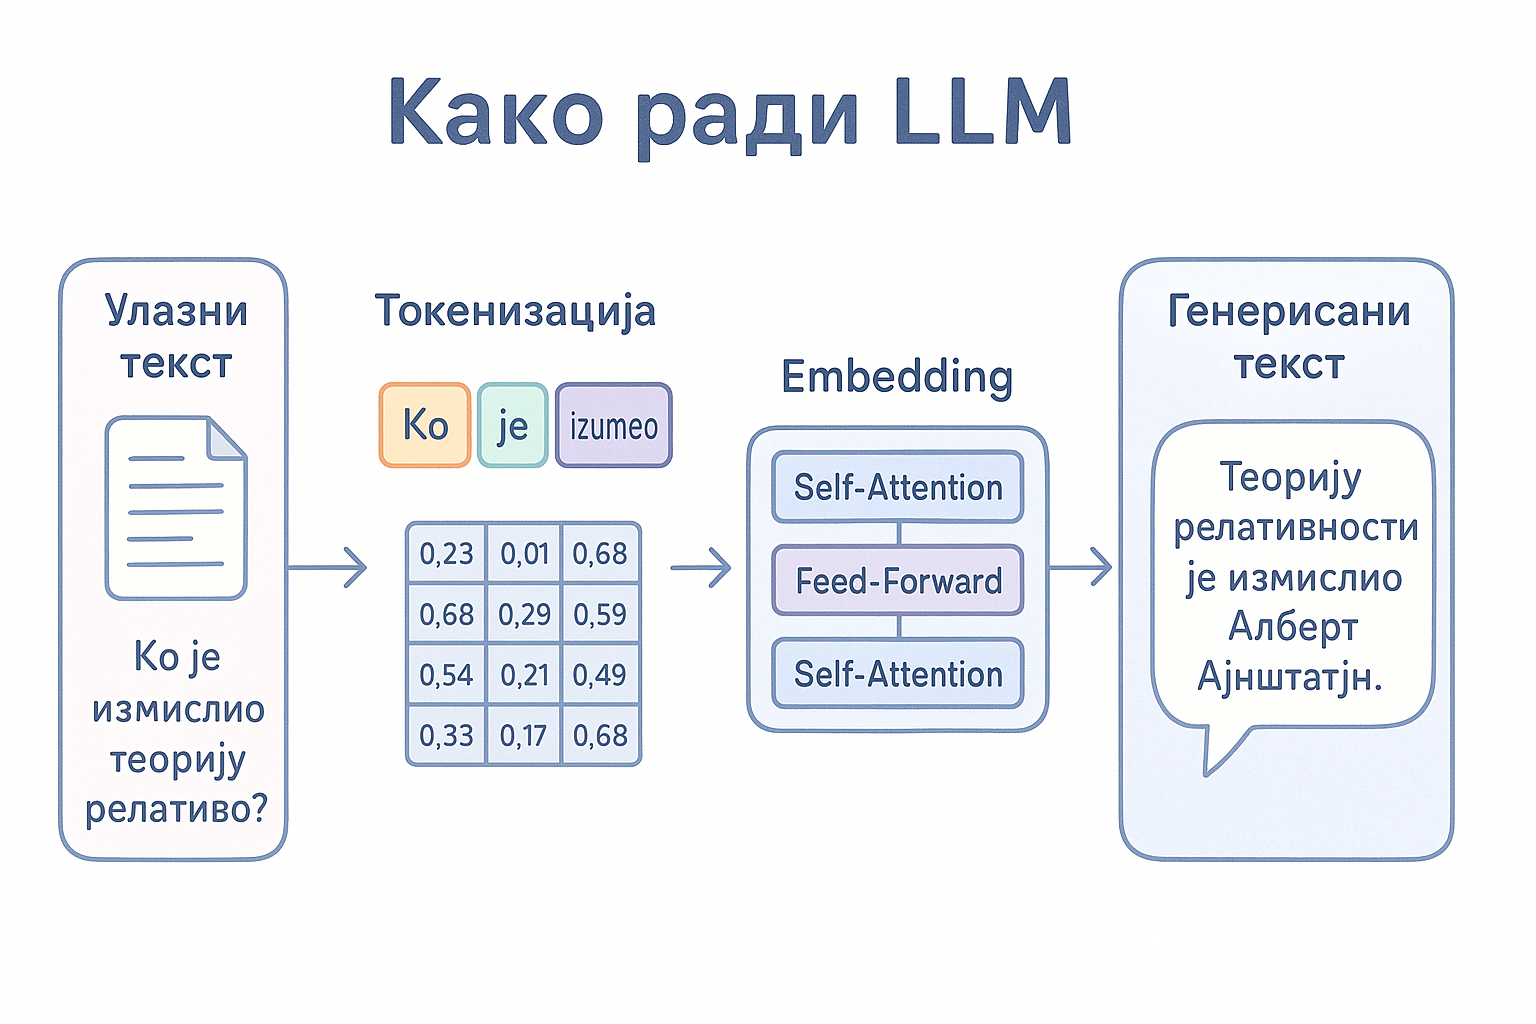
\includegraphics[width=0.8\textwidth]{slike/04/LLM_slikovito.png}
    \caption{Приказ рада LLM система}
    \label{fig:04-11}
\end{figure}
\noindent
Када у n8n-у пошаљете захтев ка OpenAI API-ју, ви заправо шаљете текст њиховом \textit{извршном фајлу} на серверу. Тај фајл консултује \textit{fajl sa parametrima} (GPT-4.1 модел), врши милионе математичких операција у милисекунди и враћа резултат. Разумевање ове поделе је важно јер објашњава зашто су јачи модели спорији и скупљи – они захтевају учитавање већих фајлова са параметрима и обављање више математичких операција за сваку генерисану реч.

\subsection{Механизам закључивања: Предикција наредног токена}

Једна од најчешћих заблуда у јавном дискурсу о вештачкој интелигенцији је антропоморфизација LLM-а – приписивање људских особина машини. Императив је разумети: Велики језички модел не поседује когнитивни апарат за разумевање текста, логике или истине. Он не зна чињенице на онтолошки начин на који их знају људи.
LLM је, у својој суштини, софистицирана статистичка машина за предвиђање (Auto-regressive Model). Његова једина функција је израчунавање вероватноће појављивања наредног симбола (токена) у низу, базирано искључиво на математичким обрасцима уоченим током тренинга на петабајтима текста.
Процес генерисања одговора није креативан чин, већ серија пробабилистичких калкулација које се одвијају секвенцијално, токен по токен.

\subsubsection{Студија случаја: Пробабилистичка дистрибуција}

Да бисмо илустровали овај механизам, анализираћемо једноставан лингвистички упит. Претпоставимо да моделу пошаљемо улазни промпт:
\begin{center}
\textit{"Ajfelov toranj se nalazi u..."}
\end{center}

У тренутку када модел прими овај низ, он не визуализује металну структуру у Паризу. Уместо тога, он врши следеће операције:
\begin{enumerate}
    \item \textbf{Анализа контекста:} Модел анализира токене Ајфелов, торањ, се, налази, у.
    \item \textbf{Претрага образаца:} Консултује своје интерне параметре (тежине) да види које речи су се у његовим тренинг подацима (књигама, википедији, чланцима) најчешће појављивале након ове специфичне секвенце.
    \item \textbf{Израчунавање вероватноће:} Модел додељује проценат вероватноће свакој речи у свом речнику (који може садржати преко 50.000 токена).
\end{enumerate}

Резултат ове операције је листа вероватноћа (дистрибуција):

\begin{itemize}
    \item \textbf{Паризу} $\rightarrow$ \textbf{97.4\%} (Висока семантичка и фактичка корелација у тренинг подацима).
    \item \textbf{Француској} $\rightarrow$ \textbf{2.1\%} (Граматички исправно, али се ређе користи у овом специфичном фразеолошком контексту).
    \item \textbf{центру} $\rightarrow$ \textbf{0.3\%} (Могућ наставак: "...центру Париза").
    \item \textbf{Лондону} $\rightarrow$ \textbf{0.001\%} (Статистичка аномалија или помињање у контексту поређења).
    \item \textbf{сендвичу} $\rightarrow$ \textbf{0.00001\%} (Потпуно одсуство семантичке везе).
\end{itemize}

Модел затим примењује алгоритам узорковања (Sampling) и бира токен са највишим скором – у овом случају Паризу.
Затим се тај нови токен додаје на крај реченице, и процес се понавља за следећу реч.

\textbf{Кључна импликација за инжењеринг:}
Овај механизам објашњава зашто модели могу да лажу самоуверено. Ако је модел трениран на хипотетичком скупу података где у 90\% текстова пише да је Ајфелов торањ у Берлину, модел би са високом вероватноћом предвидео Берлину. За модел, \textbf{истина није усклађеност са реалношћу, већ усклађеност са тренинг подацима.}
\subsubsection{Контрола креативности: Параметар Temperature}

У n8n чворовима за AI, често ћете видети поље \textbf{Temperature}. Ово је директна контрола над механизмом предвиђања који смо управо описали.

\begin{tcolorbox}[colback=blue!5!white,colframe=blue!75!black,title=Podešavanje Temperature]
\begin{itemize}
    \item \textbf{Ниска температура (0.0 - 0.3):} Модел је конзервативан. Увек бира реч са највећом вероватноћом.
    \textit{Koristiti za:} Екстракцију података, кодирање, фактуре, JSON излаз. Желимо прецизност, не изненађења.
    
    \item \textbf{Висока температура (0.7 - 1.0):} Модел постаје „креативан“. Понекад ће намерно изабрати реч са мањом вероватноћом да би текст звучао разноврсније.
    \textit{Koristiti za:} Писање блогова, маркетинг слогана, креативно писање.
\end{itemize}
\end{tcolorbox}

\subsection{Процес тренинга великих језичких модела}

Процес иницијалног тренинга великог језичког модела, познат као \textbf{pre-training}, представља фундаменталну фазу у настанку ових система и чини основу свих њихових каснијих способности. У овој фази модел се не тренира за конкретан задатак, домен или апликацију, већ стиче опште знање о језику, структури текста и обрасцима људске комуникације. Pre-training се може посматрати као процес у коме се неуронска мрежа излаже огромној количини текстуалних података како би научила статистичке и семантичке законитости које важе у природном језику.

Са инжењерског становишта, pre-training представља проблем оптимизације изузетно високих димензија. Савремени модели садрже десетине или стотине милијарди параметара, а сваки од тих параметара учествује у формирању излаза модела. Циљ тренинга је пронаћи такву конфигурацију параметара која минимизује укупну грешку на целокупном скупу података, односно која омогућава моделу да са што већом вероватноћом предвиди наредни елемент у секвенци текста.

\subsubsection{Формулација задатка: предикција наредног токена}

Основни тренинг задатак у pre-training фази своди се на проблем предикције наредног токена (енг. \textit{next-token prediction}). Текстуални улаз се најпре дели на мање јединице — токене — који могу представљати речи, делове речи, симболе или чак појединачне карактере. Модел добија секвенцу токена и у сваком кораку има задатак да процени вероватноћу сваког могућег наредног токена из унапред дефинисаног вокабулара.

Формално, модел учи апроксимацију условне вероватноће:

\[
P(t_{n+1} \mid t_1, t_2, \dots, t_n)
\]

где $t_i$ представљају токене у секвенци. Иако овај задатак на први поглед делује једноставно, његова последица је изузетно моћна: да би успешно предвидео наредни токен, модел мора имплицитно да разуме граматику, значење речи, контекст, стил писања, као и шире семантичке односе у тексту.

\subsubsection{Један тренинг корак и оптимизација}

Током тренинга, модел пролази кроз следећи циклус који се понавља огроман број пута:

Најпре се улазна секвенца токена пропагира унапред кроз неуронску мрежу (енг. \textit{forward pass}), при чему се на излазу добија дистрибуција вероватноћа над свим могућим наредним токенима. Затим се ова дистрибуција пореди са стварним токеном који се појављује у подацима. Разлика између предвиђене и стварне вредности мери се функцијом грешке, најчешће \textit{cross-entropy loss} функцијом.

Добијена грешка се потом пропагира уназад кроз мрежу (енг. \textit{backpropagation}), чиме се израчунава колико је сваки појединачни параметар допринео укупној грешци. На основу тог сигнала, параметри се коригују у веома малим корацима коришћењем варијанти градијентног спуста (нпр. алгоритми Adam или AdamW оптимизатора). Ове корекције су микроскопске, али се њихов ефекат акумулира кроз огроман број итерација.

Важно је истаћи да у овом процесу модел не добија експлицитне инструкције о значењу речи, правилима језика или логици. Све те способности се појављују као резултат статистичке оптимизације над великим бројем примера.

\subsubsection{Природа наученог знања}

Знање које модел стиче током pre-training фазе није експлицитно запамћено у облику база података или правила. Уместо тога, оно је имплицитно кодирано у тежинама неуронске мреже. То значи да се информације не могу једноставно „прочитати“ из модела, већ се испољавају кроз понашање модела током генерисања текста.

Овакав облик знања има неколико кључних карактеристика. Прво, оно је дистрибуирано — ниједан појединачни параметар не садржи одређену чињеницу, већ се информације појављују као резултат интеракције великог броја параметара. Друго, знање је апроксимативно и пробабилистичко, што објашњава зашто модели могу правити грешке или генерисати нетачне информације, али и зашто су способни за генерализацију на нове, невиђене примере.

Због тога се често каже да велики језички модели не „памте“ интернет, већ да га компресују у облику високо-димензионалног математичког простора. Ова компресија је са губитком (\textit{lossy}), слично као код JPEG компресије слике: задржавају се обрасци и структура, али не и сваки појединачни детаљ.

Један од најзанимљивијих аспеката pre-training фазе је појава тзв. специјалних способности. Како се величина модела и количина података повећавају, модел изненада почиње да показује понашања која нису била експлицитно тренирана, као што су основно резоновање, решавање математичких проблема, праћење инструкција или чак генерисање програмског кода.

Ове способности се не појављују линеарно са растом модела, већ често нагло, након преласка одређеног прага у броју параметара или количини података. Ово указује на то да pre-training не учи само локалне обрасце језика, већ гради апстрактне репрезентације које омогућавају сложеније облике когнитивног понашања.

\subsubsection{Ограничења pre-training фазе}

Иако је pre-training кључан за перформансе великих језичких модела, он има и своја ограничења. Модели тренирани искључиво на овом принципу немају експлицитно разумевање циљева корисника, етичких норми или контекста употребе. Такође, њихово знање је статично и ограничено временским периодом обухваћеним тренинг подацима.
Због тога се pre-training у пракси готово увек надопуњује додатним фазама, као што су fine-tuning на специфичним задацима, генерисање синтетичких инструкција (Self-Instruct)~\cite{wang2023selfinstruct} и усклађивање са људским преференцама (нпр. RLHF~\cite{ouyang2022,bai2022} или Direct Preference Optimization)~\cite{rafailov2023dpo}. Међутим, без снажне и обимне pre-training фазе, ове касније фазе не би имале стабилну основу на којој могу да граде додатне способности.
Pre-training представља темељ на којем почива целокупно понашање великих језичких модела. Он трансформише сирове текстуалне податке у општу језичку и семантичку компетенцију, омогућавајући моделима да функционишу као универзални алати за обраду и генерисање језика.

\subsection{Fine-Tuning: Специјализација и доменска адаптација}

Иако су велики језички модели тренирани на огромном корпусу општег знања, они су по својој природи генералисти. У специфичним инжењерским применама, често се јавља потреба да модел усвоји специфичан жаргон, формат излаза или стил комуникације који није био заступљен у иницијалном тренингу. Ту наступа процес финог подешавања (енг. \textit{Fine-Tuning})~\cite{ouyang2022,hu2022lora}.

Ако процес иницијалног тренинга (pre-training) посматрамо као стицање општег образовања, где модел учи синтаксу, логику и опште чињенице о свету, онда је fine-tuning еквивалентан специјалистичкој стручној обуци. Модел не учи како да говори, већ како да одговара у контексту специфичне организације или индустрије.

\subsubsection{Технички процес и примена}
Процес подразумева наставак тренинга модела на мањем, висококвалитетном скупу података, специфичном за домен примене. Овај метод спада у домен надгледаног учења (енг. \textit{Supervised Learning}), где се користе парови података у формату "Улаз $\rightarrow$ Жељени Излаз".

Кључни сценарији примене укључују:
\begin{itemize}
    \item \textbf{Стилска и тонална адаптација:} Тренирање модела на корпоративној архиви комуникације како би генерисани одговори рефлектовали специфичан начин генерисања одговора, терминологију и форматирање.
    \item \textbf{Структурална усклађеност:} Тренирање модела да конзистентно генерише излаз у специфичним, често нестандардним форматима (нпр. власнички XML шеме или специфични JSON формати), чиме се минимизира ризик од грешака при парсирању.
    \item \textbf{Оптимизација ресурса:} Мањи модел (нпр. 7 милијарди параметара) који је фино подешен за један специфичан задатак често може надмашити перформансе гигантског модела (GPT-4.1), уз драстично мање трошкове инференције и мању латенцију~\cite{chen2023frugal,hu2022lora}.
\end{itemize}

\begin{tcolorbox}[colback=green!5!white,colframe=green!75!black,title=Arhitektonska dilema: RAG ili Fine-Tuning?]
У пројектовању AI система, инжењери морају направити избор између две методологије побољшања перформанси:
\begin{itemize}
    \item \textbf{RAG (Retrieval-Augmented Generation):} Користи се када је потребно моделу пружити \textit{novo znanje} или променљиве чињенице (нпр. тренутно стање залиха, вести). RAG функционише као отворена књига током испита.
    \item \textbf{Fine-Tuning:} Користи се када је потребно променити \textit{понашање} модела или научити га новој \textit{вештини} (нпр. специфичан начин писања кода). Сликовито, fine-tuning мења синапсе у мозгу модела.
\end{itemize}
У пракси, најробуснији системи често користе хибридни приступ.
\end{tcolorbox}

На слици~\ref{fig:04-12} дат је илустративни приказ тренинга модела по свакој фази.


\begin{figure}[h!]
    \centering
    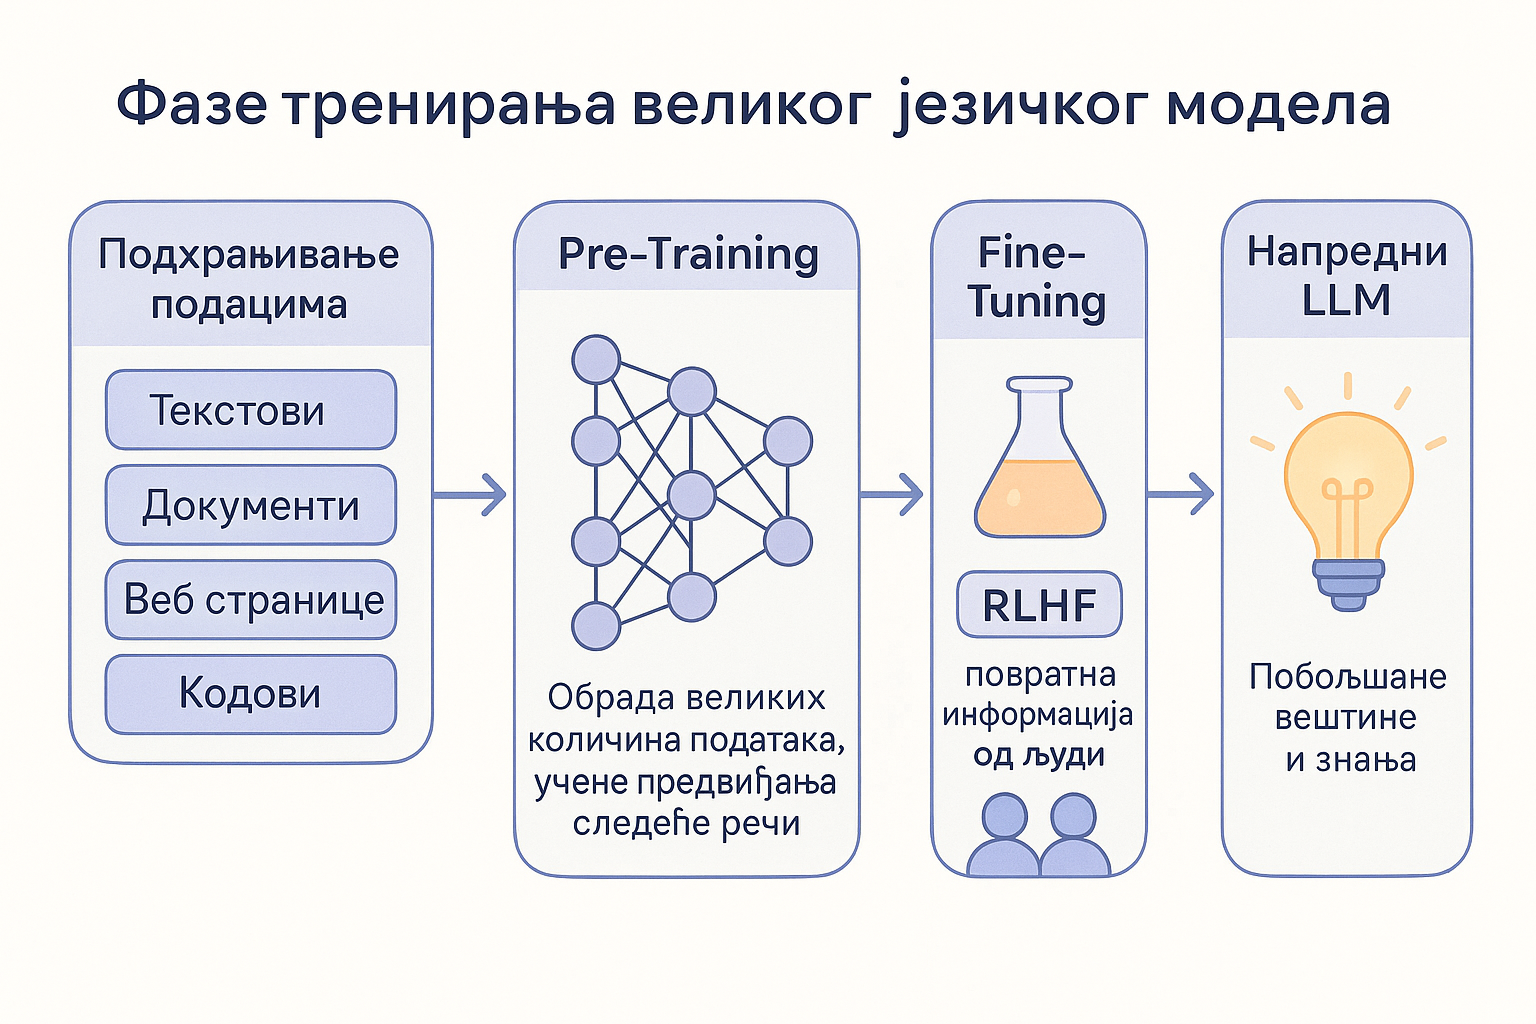
\includegraphics[width=0.95\textwidth]{slike/04/treniranje_modela.png}
    \caption{Илустрација процеса тренинга модела}
    \label{fig:04-12}
\end{figure}



\subsection{Трансформативна улога: Од генератора текста до Аутономног Агента}

Најзначајнија еволуција у примени LLM технологије огледа се у транзицији са парадигме пасивног \textit{AI Asistenata-a} на парадигму активног \textit{Agenta}.

Сами по себи, LLM-ови су изоловани системи за обраду текста, без директне везе са спољним светом. Међутим, када се интегришу у шире софтверске системе путем API интерфејса, они добијају способност перцепције и деловања.

\subsubsection{Механизам оперативног деловања}
Фундаментално питање гласи: \textit{Како пробабилистички модел, који само предвиђа наредну реч, може управљати детерминистичким софтверским системима?} Одговор лежи у механизму позивања функција (енг. \textit{Function Calling}) и генерисању структурираних података.

Процес доношења одлука у агентској архитектури одвија се кроз следеће фазе:

\begin{enumerate}
    \item \textbf{Детекција намере (енг. \textit{Intent Recognition}):} Корисник упућује захтев природним језиком (нпр. "Закажи састанак са клијентом Х за сутра у 10х").
    \item \textbf{Расудивање и формулација команде:} LLM анализира захтев и, уместо генерисања конверзацијског одговора, конструише структурирани објекат (најчешће у JSON формату) који представља инструкцију за екстерни систем.
    \\
    \begin{lstlisting}[language=json, basicstyle=\ttfamily\scriptsize, caption={Primer strukturirane instrukcije koju generiše Agent}]
    {
      "service": "calendar_api",
      "operation": "create_event",
      "payload": {
        "title": "Meeting with Client X",
        "datetime": "2024-10-25T10:00:00Z",
        "duration_minutes": 60,
        "attendees": ["client@example.com"]
      }
    }
    \end{lstlisting}
    
    \item \textbf{Извршење (Execution Runtime):} Контролни софтвер (бекенд систем) детектује овај структурирани излаз, валидира га и извршава стварни API позив ка циљном сервису (нпр. календару или бази података).
    \item \textbf{Повратна спрега (Feedback Loop):} Резултат извршења (успех или грешка) враћа се моделу као нови улазни податак. Модел затим генерише финални одговор кориснику („Састанак је успешно заказан“).
\end{enumerate}

У овој архитектури, LLM преузима улогу когнитивног контролера. Он не врши саму радњу (не шаље мрежне пакете), већ оркестрира алате. Његова функција је превођење нејасних, неструктурираних људских намера у прецизне, машински читљиве инструкције. Ово је суштина агентске технологије: премошћавање јаза између флексибилности људског језика и ригидности софтверских API-ја.

% =================================================================================
% POGLAVLJE 4
% =================================================================================

% =================================================================================
% POGLAVLJE 5
% =================================================================================

\section{Алати за развој аутоматизације: Платформа n8n}

У претходним поглављима разматрани су концептуални и архитектонски темељи
AI аутоматизације: референтна слојевита архитектура, таксономија AI система,
као и унутрашњи механизми великих језичких модела. Сада се фокус пребацује
са теоријских оквира на конкретан инжењерски алат кроз који се ови концепти
могу практично реализовати. За потребе овог курса, као репрезентативна
платформа за изградњу аутоматизованих и AI-оријентисаних радних токова
анализираће се платформа \textbf{n8n}.

n8n (чита се „ен–ејт–ен“, што се односи на скраћеницу појма
\textit{nodemation}, односно \textit{node-based automation})~\cite{n8n} развијена је
2019. године и представља један од најистакнутијих представника нове
генерације алата за визуелну оркестрацију процеса. За разлику од класичних
„low-code/no-code“ сервиса, који су углавном искључиво затворени и
хостовани у облаку, n8n се издваја комбинацијом отворености изворног
кода, могућности самосталног хостовања и нативне интеграције са
екосистемом великих језичких модела.

Разлози због којих се n8n користи као репрезентативна платформа у овом
курсу су тројаки:

\begin{itemize}
    \item \textbf{Репрезентативност:} n8n имплементира све кључне
    елементе референтне архитектуре из одељка~\ref{sec:tehnicka-infrastruktura} — тригере, оркестрацију,
    интеграције, податковни слој, AI слој и основни опсервациони слој.
    \item \textbf{Приступачност:} платформа је доступна бесплатно за
    самостално хостовање, што омогућава студентима и истраживачима
    експериментисање без финансијских баријера.
    \item \textbf{Едукативна транспарентност:} за разлику од потпуно
    затворених SaaS решења, код n8n-а су извршне инстанце, подаци и
    логови доступни инжењеру, што омогућава дубље разумевање рада
    аутоматизације.
\end{itemize}

Важно је нагласити да n8n у овом контексту није ексклузивни избор, већ
\textit{дидактички медиј}: принципи који се уче кроз n8n
(моделовање тока, рад са чворовима, експресије, AI интеграција)
директно су преносиви на друге платформе као што су Make (раније Интегромат),
Zapier, Microsoft Power Automate, Pipedream или Apache Airflow.

\subsection{Архитектура n8n платформе}

Са становишта софтверског инжењерства, n8n није монолитан алат,
већ скуп међусобно повезаних компоненти које заједно чине
платформу за извршавање аутоматизованих радних токова. Разумевање
унутрашње архитектуре неопходно је за правилно доношење одлука
о начину имплементације, скалабилности, безбедности и интеграције
са постојећом инфраструктуром организације.

\subsubsection{Филозофија дизајна и лиценцни модел}

n8n је развијен у складу са принципом \textbf{fair-code} лиценцирања,
прецизније под лиценцом \textit{Sustainable Use License}. Ова лиценца
представља хибридни модел између традиционалног отвореног кода и
комерцијалног софтвера, са следећим кључним карактеристикама:

\begin{itemize}
    \item Изворни код је јавно доступан, може се прегледати,
    модификовати и користити у некомерцијалне сврхе и интерне
    пословне потребе организације.
    \item Дистрибуција модификованих верзија као конкурентског
    производа није дозвољена, чиме се штите економски интереси
    матичне компаније.
    \item Корисници могу самостално хостовати платформу без плаћања
    лиценце, што је посебно значајно за организације са рестриктивним
    политикама заштите података.
\end{itemize}

Овакав модел омогућава баланс између транспарентности и одрживости
развоја платформе, чиме се избегава класична дилема између
искључиво отворених и искључиво комерцијалних решења.

\subsubsection{Технолошки стек}

Са техничке стране, n8n је развијен у програмском језику
\textbf{TypeScript} и извршава се у \textbf{Node.js} окружењу.
Овај избор има неколико важних последица:

\begin{itemize}
    \item \textbf{Асинхрони модел извршавања:} Node.js природно
    подржава асинхроне операције, што одговара природи аутоматизације
    где се највећи део времена троши на чекање одговора од екстерних
    сервиса (API позиви, базе података).
    \item \textbf{Богат екосистем пакета:} преко \textit{npm} репозиторијума,
    n8n може искористити хиљаде постојећих библиотека за рад са различитим
    протоколима и форматима.
    \item \textbf{Проширивост у JavaScript-у:} кориснички Code чворови
    пишу се у JavaScript-у (и опционо Python-у кроз \textit{Pyodide}
    рунтиме), што омогућава директно проширење функционалности без
    напуштања платформе.
\end{itemize}

Frontend (визуелни едитор) имплементиран је као Single-Page Application
заснована на \textit{Vue.js} оквиру, док је backend организован као
модуларна колекција сервиса одговорних за извршавање, перзистенцију
и аутентификацију.

\subsubsection{Модели имплементације}

n8n се може инсталирати и користити у неколико различитих модела,
од којих сваки има специфичне предности и ограничења:

\paragraph{n8n Cloud (Managed service)}
Комерцијална верзија у којој n8n тим управља целокупном инфраструктуром.
Корисник се пријављује, креира радне токове и не брине о серверима,
ажурирањима или резервним копијама. Овај модел је погодан за:
брзе прототипове, мање организације без DevOps капацитета и сценарије
где подаци нису строго поверљиви.

\paragraph{Self-hosted (Самостално хостовање)}
Најчешћи начин коришћења у академским и пословним окружењима.
n8n се дистрибуира као \textit{Docker} контејнер, што омогућава
једноставно покретање на било којој инфраструктури која подржава
контејнере. Типично размештање обухвата:

\begin{itemize}
    \item n8n апликацијски сервер (Node.js процес),
    \item перзистентну базу података (\textit{SQLite} за развој,
    \textit{PostgreSQL} или \textit{MySQL} за продукцију),
    \item опционално \textit{Redis} за queue мод (скалирано извршавање),
    \item reverse proxy (\textit{nginx}, \textit{Traefik}) за HTTPS
    терминацију и webhook рутирање.
\end{itemize}

\paragraph{Embedded (Угњеждено)}
n8n се може интегрисати и као библиотека у оквиру других апликација,
чиме постаје уграђени мотор за аутоматизацију. Овај модел је релативно
редак и користи се у специјализованим производима који желе да својим
корисницима понуде визуелну изградњу токова без развоја сопственог
система од нуле.

\subsubsection{Главне компоненте система}

Без обзира на модел имплементације, интерна архитектура n8n-а
састоји се од неколико логички раздвојених компоненти:

\begin{enumerate}
    \item \textbf{Едитор UI:} визуелно окружење у којем корисник
    гради и визуализује радне токове. Представља слој презентације
    и не учествује директно у извршавању.
    \item \textbf{Workflow Engine:} централни мотор који интерпретира
    граф чворова, управља током података, редоследом извршавања
    и стањем тренутне инстанце.
    \item \textbf{Node Runtime:} извршно окружење за појединачне
    чворове. Сваки чвор је у суштини функција која прима улаз,
    обавља операцију и враћа излаз.
    \item \textbf{Persistence Layer:} слој базе података у којем се
    чувају дефиниције радних токова, креденцијали (енкриптовани),
    историја извршавања и конфигурација.
    \item \textbf{Webhook Server:} подсистем који прима долазне HTTP
    захтеве и покреће одговарајуће радне токове.
    \item \textbf{Scheduler:} интерни сервис за покретање радних
    токова према временском распореду.
    \item \textbf{Queue Worker (опционо):} у скалираним инсталацијама,
    извршавање радних токова се делегира посебним worker процесима
    који преузимају послове из Redis реда.
\end{enumerate}

\subsubsection{Позиционирање у односу на конкуренцију}

У категорији workflow аутоматион алата постоји неколико доминантних
платформи са којима се n8n најчешће пореди. Табела~\ref{tab:04-3}
приказује поједностављени компаративни преглед.

\begin{table}[h!]
\centering
\caption{Поређење n8n са сродним платформама за аутоматизацију}
\vspace{0.3cm}
\begin{adjustbox}{max width=\textwidth}
\begin{tabular}{|p{3.2cm}|p{2.7cm}|p{2.7cm}|p{2.7cm}|}
\hline
\textbf{Карактеристика} & \textbf{n8n} & \textbf{Zapier} & \textbf{Make} \\
\hline
Self-hosting & Да & Не & Не \\
\hline
Приступ изворном коду & Да (fair-code) & Не & Не \\
\hline
Ценовни модел & По извршавању радног тока & По задатку & По операцији \\
\hline
Code чворови & JavaScript / Python & Ограничено & JavaScript \\
\hline
Нативна AI интеграција & LangChain.js & Делимично & Делимично \\
\hline
Комплексне гранања & Напредније & Линеарније & Напредније \\
\hline
\end{tabular}
\end{adjustbox}
\label{tab:04-3}
\end{table}

Кључна предност n8n-а у поређењу са Zapier-ом јесте могућност
самосталног хостовања, док је у поређењу са Make платформом
n8n флексибилнији у смислу програмабилности и контроле над
извршним окружењем. Са друге стране, чисто визуелно искуство и
број готових интеграција често су зрелији код комерцијалних
конкурената.

\subsection{Структура радног тока (Workflow)}

Централни појам у n8n платформи јесте \textbf{радни ток}
(енг. \textit{workflow}). Са формалне стране, радни ток се може
описати као усмерени ациклични граф (енг. \textit{Directed Acyclic
Graph, DAG}), где:

\begin{itemize}
    \item \textbf{чворови} (\textit{nodes}) представљају појединачне
    операције (нпр. читање емаил-а, позив API-ја, трансформација
    података, позив LLM-а),
    \item \textbf{ивице} (\textit{connections}) представљају ток
    података између чворова,
    \item не сме постојати циклус у графу — ако је итеративно
    понашање потребно, оно се моделује кроз експлицитне Лооп или
    Суб-workflow конструкте.
\end{itemize}

Иако визуелно делује као дијаграм тока, n8n граф није чисто
контролни ток као у класичном програмирању, већ примарно
\textbf{ток података} (\textit{dataflow}) — свака веза преноси
структурисане податке из једног чвора у следећи.

\subsubsection{Податковни модел: рад са ставкама}

Једна од фундаменталних концептуалних разлика у односу на
традиционално програмирање јесте чињеница да n8n ради са
\textbf{низовима ставки} (енг. \textit{items}), а не са појединачним
вредностима. Свака ставка је JSON објекат облика:

\begin{lstlisting}[language=json, caption={Struktura stavke u n8n}]
{
  "json": {
    "id": 42,
    "email": "kupac@example.com",
    "iznos": 1500
  },
  "binary": { /* opcionalno: fajlovi, slike */ }
}
\end{lstlisting}

Када чвор прими 100 ставки као улаз, он се по подразумеваном
понашању извршава 100 пута — једном по свакој ставки. Овај
имплицитни „лооп“ је последица чињенице да се подаци у
аутоматизацији најчешће јављају у баженим облицима (листа
наруџбина, листа корисника, листа порука) и да се над сваком
ставком понавља иста операција.

Овакав податковни модел доноси неколико важних последица:

\begin{itemize}
    \item \textbf{Имплицитна паралелизација:} чвор не мора експлицитно
    да итерира кроз листу, већ се исти код аутоматски примењује на
    сваку ставку.
    \item \textbf{Хетерогеност ставки:} свака ставка може имати
    другачију структуру, што захтева пажљиво руковање када се
    очекује конзистентност.
    \item \textbf{Спајање и раздвајање токова:} помоћу чворова
    \textit{Merge} и \textit{Split In Batches} могуће је мењати
    грануларност обраде.
\end{itemize}

\subsubsection{Expressions и динамичке вредности}

Конфигурација чворова у n8n-у ретко је статичка. Најчешће се
вредности поља израчунавају динамички, на основу излаза претходних
чворова. За то служи систем \textbf{експресија} (\textit{expressions})
који користи поједностављени JavaScript синтаксни модел унутар
ознака \texttt{\{\{ \}\}}~\cite{n8n}.

Типични примери експресија:
\begin{itemize}
    \item \texttt{\{\{ \$json.email \}\}} — приступ пољу тренутне ставке,
    \item \texttt{\{\{ \$node["HTTP Request"].json.id \}\}} — приступ
    излазу конкретног претходног чвора,
    \item \texttt{\{\{ \$now.format("yyyy-MM-dd") \}\}} — коришћење
    помоћних функција (датуми, стрингови, бројеви),
    \item \texttt{\{\{ \$items().length \}\}} — агрегатне операције
    над целим низом ставки.
\end{itemize}

Expressions омогућавају да се логика писања кода замени
декларативним конфигурисањем, што значајно снижава праг уласка
за нетехничке кориснике, а истовремено задржава пуну флексибилност
за напредне сценарије.

\subsubsection{Типови чворова}

Са становишта архитектуре извршавања, чворови у n8n-у деле се
на три основне категорије:

\begin{enumerate}
    \item \textbf{Trigger чворови:} иницирају извршавање радног тока.
    Сваки workflow мора имати барем један триггер чвор.
    \item \textbf{Регулар (Action) чворови:} обављају операције
    над подацима — позиви API-ја, трансформације, логичке одлуке,
    писање у базу и слично.
    \item \textbf{Суб-workflow чворови:} омогућавају модуларност
    позивањем другог радног тока као функције, чиме се постиже
    декомпозиција сложених система.
\end{enumerate}

\subsection{Trigger чворови (Окидачи)}

Trigger чворови представљају улазну тачку сваког аутоматизованог
процеса. Њихова улога је да \textit{детектују догађај} и покрену
извршавање радног тока. У зависности од природе догађаја који
их активира, тригери се могу класификовати у неколико група.

\subsubsection{Мануални тригери}

Најједноставнији облик окидача, који се користи готово искључиво
током развоја и тестирања. Корисник експлицитно кликом у едитору
покреће извршавање. Мануални тригер нема механизам за покретање
у продукционом окружењу и служи превасходно као развојни алат.

\subsubsection{Временски тригери (Schedule / Cron)}

Временски тригери покрећу радни ток према унапред дефинисаном
распореду. Конфигурисање се врши или кроз поједностављени интерфејс
(нпр. „сваких 15 минута“, „сваког понедељка у 09:00“) или кроз
класичну \textit{cron} синтаксу за сложеније обрасце.

Типични сценарији употребе:
\begin{itemize}
    \item дневни извештаји у одређено време,
    \item периодична провера стања екстерних сервиса,
    \item batch обрада података током ноћи,
    \item слање подсетника корисницима.
\end{itemize}

\subsubsection{Webhook тригери}

Webhook тригери су HTTP ендпоинт-и које n8n експонира спољном
свету. Када екстерни систем пошаље HTTP захтев на тај ендпоинт,
радни ток се тренутно покреће. Овај модел омогућава реакцију у
реалном времену (латенција у милисекундама) и представља основу
за интеграцију са модерним SaaS апликацијама.

Разликујемо два мода webhook тригера:
\begin{itemize}
    \item \textbf{Синхрони мод:} клијент који је позвао webhook чека
    на одговор радног тока. Погодан када је резултат обраде неопходан
    позиваоцу (нпр. AI агент који враћа одговор кориснику).
    \item \textbf{Асинхрони мод:} радни ток одмах враћа потврду
    пријема, док се обрада наставља у позадини. Погодан за
    дуготрајне процесе где клијент не треба да чека.
\end{itemize}

\subsubsection{Polling и app-specific тригери}

Велика већина апликацијски-специфичних тригера (Gmail, Slack, Notion,
Google Drive и сл.) интерно функционише или кроз прави webhook
механизам (када га екстерна апликација подржава) или кроз
\textit{polling} — периодичну проверу стања кроз API. Иако је
polling технички мање ефикасан и уноси латенцију, он је често
једина опција за сервисе који не подржавају излазне webhook-е.

\subsection{Регулар (Action) чворови}

Регулар чворови чине највећи део сваког нетривијалног радног тока.
Они се могу груписати у неколико логичких категорија према својој
улози.

\subsubsection{Интеграциони чворови}

Највећи број n8n чворова представљају \textit{integracije} —
унапред упаковани конектори за конкретне сервисе (Gmail, Slack,
HubSpot, Salesforce, Notion, PostgreSQL итд.). Сваки интеграциони
чвор апстрахује детаље API комуникације и излаже кориснику
декларативан интерфејс за избор операција (нпр. „пошаљи поруку“,
„креирај запис“, „претражи контакте“).

Када готов конектор не постоји, користи се универзални
\textbf{HTTP Рекуест} чвор који омогућава директан позив било
ког REST или GraphQL API-ја. Ово практично значи да n8n може
комуницирати са апсолутно сваким системом који излаже неки облик
HTTP интерфејса.

\subsubsection{Логички чворови}

За управљање током извршавања користе се посебни логички
чворови:

\begin{itemize}
    \item \textbf{IF:} бинарно гранање на основу услова
    (једнако, садржи, веће од и сл.).
    \item \textbf{Switch:} вишесмерно гранање са до четири или више
    излазних путања, на основу вредности поља.
    \item \textbf{Merge:} спајање више грана у једну, са различитим
    стратегијама (по индексу, по кључу, додавањем).
    \item \textbf{Loop / Split In Batches:} експлицитно итерирање
    кроз ставке у мањим групама, корисно за рад са великим скуповима
    података и за поштовање API рате-лимит-а.
    \item \textbf{Wait:} паузирање извршавања на одређено време или
    до наступања екстерног догађаја, што омогућава дуготрајне токове
    са „human-in-the-loop“ елементима.
\end{itemize}

\subsubsection{Чворови за трансформацију података}

Реални радни токови готово увек захтевају трансформацију података
између различитих система. За то служе специјализовани чворови:

\begin{itemize}
    \item \textbf{Set / Edit Fields:} додавање, брисање или
    преименовање поља на ставкама.
    \item \textbf{Code (JavaScript/Python):} писање произвољне
    логике када декларативни чворови нису довољни.
    \item \textbf{Aggregate:} груписање ставки по кључу и
    израчунавање агрегатних вредности.
    \item \textbf{Item Lists:} операције над низовима
    (сортирање, дедупликација, избор потскупа).
\end{itemize}

\subsection{AI интеграција: нативна подршка за LangChain}

Од 2023. године, n8n је увео нативну интеграцију са
\textit{LangChain.js} библиотеком~\cite{langchain}, чиме је платформа постала
један од првих визуелних алата са потпуним уградним оквиром
за изградњу AI агената. Ова интеграција није само додатак,
већ засебна категорија чворова означена као \textbf{AI Нодес}.

\subsubsection{Типови AI чворова}

LangChain интеграција у n8n организована је кроз неколико
специјализованих група чворова:

\begin{itemize}
    \item \textbf{AI Agent чвор:} централни извршни чвор који
    имплементира агентску петљу (Thought–Action–Observation),
    описану у одељку~\ref{sec:taksonomija-ai}. Агент прихвата кориснички промпт и
    аутономно одлучује које алате (Tool чворове) да позове.
    \item \textbf{Chat Model чворови:} апстракције за конкретне
    LLM провајдере — OpenAI, Anthropic, Google Gemini, Mistral,
    као и локалне моделе кроз \textit{Ollama} или \textit{LM Studio}.
    \item \textbf{Memory чворови:} имплементација краткорочне и
    дугорочне меморије агента — buffer меморија (последњих
    \textit{n} порука), summary меморија (сажетак конверзације),
    vector меморија (семантичко памћење).
    \item \textbf{Tool чворови:} алати које агент може позивати —
    Calculator, Wikipedia, HTTP Request, или било који други
    n8n чвор обучен у tool wrapper.
    \item \textbf{Vector Store чворови:} интеграција са векторским
    базама (\textit{Pinecone, Qdrant, Weaviate, Supabase, Postgres
    pgvector}) као основа RAG архитектуре.
    \item \textbf{Document Loader и Text Splitter чворови:}
    помоћни чворови за припрему докумената пре векторизације.
\end{itemize}

\subsubsection{Модуларност агентске архитектуре}

Посебност n8n приступа AI агентима јесте што су појединачне
компоненте архитектуре (модел, меморија, алати) моделоване као
\textit{посебни чворови} који се повезују на централни AI Агент
чвор преко специфичних улазних портова. Овај дизајн има неколико
последица:

\begin{itemize}
    \item Промена LLM провајдера (нпр. са OpenAI на Anthropic)
    своди се на замену једног чвора, без измене логике агента.
    \item Меморија и алати су експлицитни и видљиви у дијаграму,
    што значајно олакшава разумевање и дебуговање.
    \item Исти агент може се позивати из више различитих радних
    токова, чиме се постиже поновна употребљивост.
\end{itemize}

\subsection{Credentials систем и безбедност}

Комуникација са екстерним сервисима захтева аутентификацију, што
отвара питање безбедног складиштења креденцијала. n8n имплементира
наменски \textbf{Credentials} подсистем са следећим својствима:

\begin{itemize}
    \item Креденцијали се чувају у бази података у
    \textbf{енкриптованом облику}, коришћењем кључа који је
    конфигурисан на нивоу инстанце (\texttt{N8N\_ENCRYPTION\_KEY}).
    \item Подржани су стандардни механизми аутентификације:
    Basic Auth, API Key, Bearer Token, OAuth1, OAuth2, JWT и
    произвољни custom HTTP заглавља.
    \item Креденцијали се могу \textbf{делити између корисника и
    тимова}, са грануларном контролом приступа.
    \item Вредности креденцијала се не приказују у логовима и
    извршној историји, чиме се спречава њихово случајно откривање.
\end{itemize}

Раздвајање конфигурације радног тока од креденцијала омогућава
и преносивост: исти workflow може се пренети из развојног у
продукционо окружење уз коришћење различитих скупова креденцијала,
без измене саме логике тока.

\subsection{Error handling, debugging и observability}

Робустност аутоматизованог система не мери се само по његовој
способности да ради у идеалним условима, већ и по начину на који
се понаша у присуству грешака. n8n нуди неколико слојева механизама
за рад са грешкама.

\subsubsection{Политике руковања грешкама на нивоу чвора}

Сваки чвор може се конфигурисати са специфичном политиком у случају
грешке:

\begin{itemize}
    \item \textbf{Stop Workflow (подразумевано):} цео радни ток се
    зауставља, а извршавање се бележи као неуспешно.
    \item \textbf{Continue on Fail:} грешка се бележи, али се
    извршавање наставља кроз алтернативну путању.
    \item \textbf{Retry on Fail:} чвор се аутоматски поново извршава
    одређени број пута, са конфигурисаним размаком (експоненцијални
    backoff).
\end{itemize}

\subsubsection{Error workflow}

Поред политика на нивоу чвора, n8n омогућава дефинисање посебног
\textbf{Error Workflow}-а — специјалног радног тока који се
аутоматски покреће сваки пут када главни workflow падне. Типична
употреба укључује слање нотификације DevOps тиму, креирање
тикета у систему за праћење грешака и логовање у екстерни
опсервациони систем (нпр. \textit{Sentry, Datadog}).

\subsubsection{Execution history и debugging}

Свако извршавање радног тока бележи се у \textbf{execution history}
где се могу прегледати улази и излази сваког чвора, статус и трајање.
Овај механизам представља основни опсервациони слој n8n платформе и
од непроцењиве је вредности током развоја и дијагностике.

Додатно, едитор поседује мод \textit{step-by-step execution} који
омогућава извршавање радног тока један чвор по чвор, са прегледом
података у сваком тренутку — аналогно класичном дебуггер-у у IDE
окружењима.

\subsection{Скалабилност и deployment}

За озбиљније продукционе примене, n8n нуди тзв. \textbf{queue mode}
архитектуру која раздваја примарну инстанцу (која прима webhook-ове и
управља сцхедулером) од једног или више \textbf{worker} процеса
који извршавају радне токове~\cite{n8n}. Комуникација између компоненти одвија
се кроз \textit{Redis} ред послова.

Овај приступ доноси следеће предности:
\begin{itemize}
    \item \textbf{Хоризонтална скалабилност:} број worker процеса
    може се динамички повећавати у зависности од оптерећења.
    \item \textbf{Отпорност на отказе:} пад једног worker-а не
    блокира примање нових окидача; незавршени послови се
    редистрибуирају.
    \item \textbf{Изолација ресурса:} дуготрајни и ресурсно захтевни
    радни токови могу се извршавати на посебним worker групама
    без утицаја на латенцију осталих.
\end{itemize}

У Kubernetes окружењима, n8n се може разместити кроз званичне
Helm chart-ове, што омогућава интеграцију са стандардним алатима
за мониторинг, autoscaling и управљање конфигурацијом.

\subsection{Пример имплементације: Интелигентна обрада корисничких тикета}

Да би се илустровала интеракција свих описаних компоненти, у наставку
се разматра реалистичан пример аутоматизације процеса корисничке
подршке. Циљ система је да сваки долазни email корисничке подршке
буде анализиран, класификован и обрађен на начин који минимизује
људски рад за рутинске случајеве, док комплексне и хитне случајеве
ескалира људском оператеру.

\subsubsection{Функционална спецификација}

Систем треба да:
\begin{enumerate}
    \item региструје сваки нови емаил упућен на адресу
    \texttt{support@firma.com},
    \item утврди тему поруке (Рачуни, Техничка подршка, Општи упит),
    \item процени емоционални тон корисника (неутралан, фрустриран,
    разјарен),
    \item за рутинске упите генерише предлог одговора ослоњен на
    базу знања компаније,
    \item за хитне или негативне случајеве ескалира тикет менаџеру
    путем Slack нотификације,
    \item у свим случајевима упише резиме у CRM систем.
\end{enumerate}

\subsubsection{Архитектура радног тока}

Имплементација се састоји од следећих чворова, повезаних у јединствен
граф:

\begin{enumerate}
    \item \textbf{Trigger чвор (Gmail Trigger):} активира се на сваку
    нову поруку. Конфигурисан као polling са интервалом од једне
    минуте.

    \item \textbf{Set чвор:} нормализује структуру података,
    издвајајући само релевантна поља: пошиљаоца, наслов, тело
    поруке и време пријема.

    \item \textbf{AI Agent чвор (Класификатор):} повезан на OpenAI
    Chat Model и конфигурисан са системским промптом који налаже
    строго структурисан JSON излаз. Пример очекиваног одговора:

\begin{lstlisting}[language=json, caption={Strukturisan izlaz klasifikacionog agenta}]
{
  "kategorija": "Tehnicka podrska",
  "ton": "frustriran",
  "hitnost": 8,
  "kratak_opis": "Korisnik ne moze da se prijavi vec dva dana"
}
\end{lstlisting}

    \item \textbf{Switch чвор:} усмерава ток извршавања у зависности
    од категорије и хитности:
    \begin{itemize}
        \item ако је хитност $\geq 7$ или је тон „разјарен“ —
        грана А (ескалација),
        \item ако је категорија „Рачуни“ — грана Б (финансије),
        \item у супротном — грана Ц (рутински одговор).
    \end{itemize}

    \item \textbf{Грана А (Ескалација) — Slack чвор:} шаље форматирано
    упозорење у канал \texttt{\#support-urgent}, уз линк ка оригиналном
    емаил-у и сажетак ситуације.

    \item \textbf{Грана Б (Финансије) — Forward + CRM:} прослеђује
    поруку финансијском тиму и аутоматски креира напомену у CRM-у.

    \item \textbf{Грана Ц (Рутински одговор) — RAG агент:} додатни AI
    агент повезан на векторску базу знања генерише предлог одговора
    утемељен у званичној документацији компаније. Овај предлог се
    \textbf{не шаље аутоматски}, већ се креира као драфт у Gmail-у,
    са нотификацијом оператеру да прегледа и одобри садржај.

    \item \textbf{Завршни чвор (PostgreSQL):} у свим гранама, на крају
    се у CRM базу уписује запис о обрађеном тикету са резултатима
    класификације и предузетим акцијама.

    \item \textbf{Error Workflow:} у случају било каквог отказа —
    недоступност OpenAI API-ја, грешка у Slack аутентификацији или
    пад базе — покреће се резервни ток који обавештава DevOps тим
    и привремено чува неуспешне ставке за каснију ручну обраду.
\end{enumerate}

На слици~\ref{fig:04-13} приказан је визуелни дијаграм описаног
радног тока, са свим главним чворовима, гранама извршавања и резервним
Error Workflow током.

\begin{figure}[h!]
    \centering
    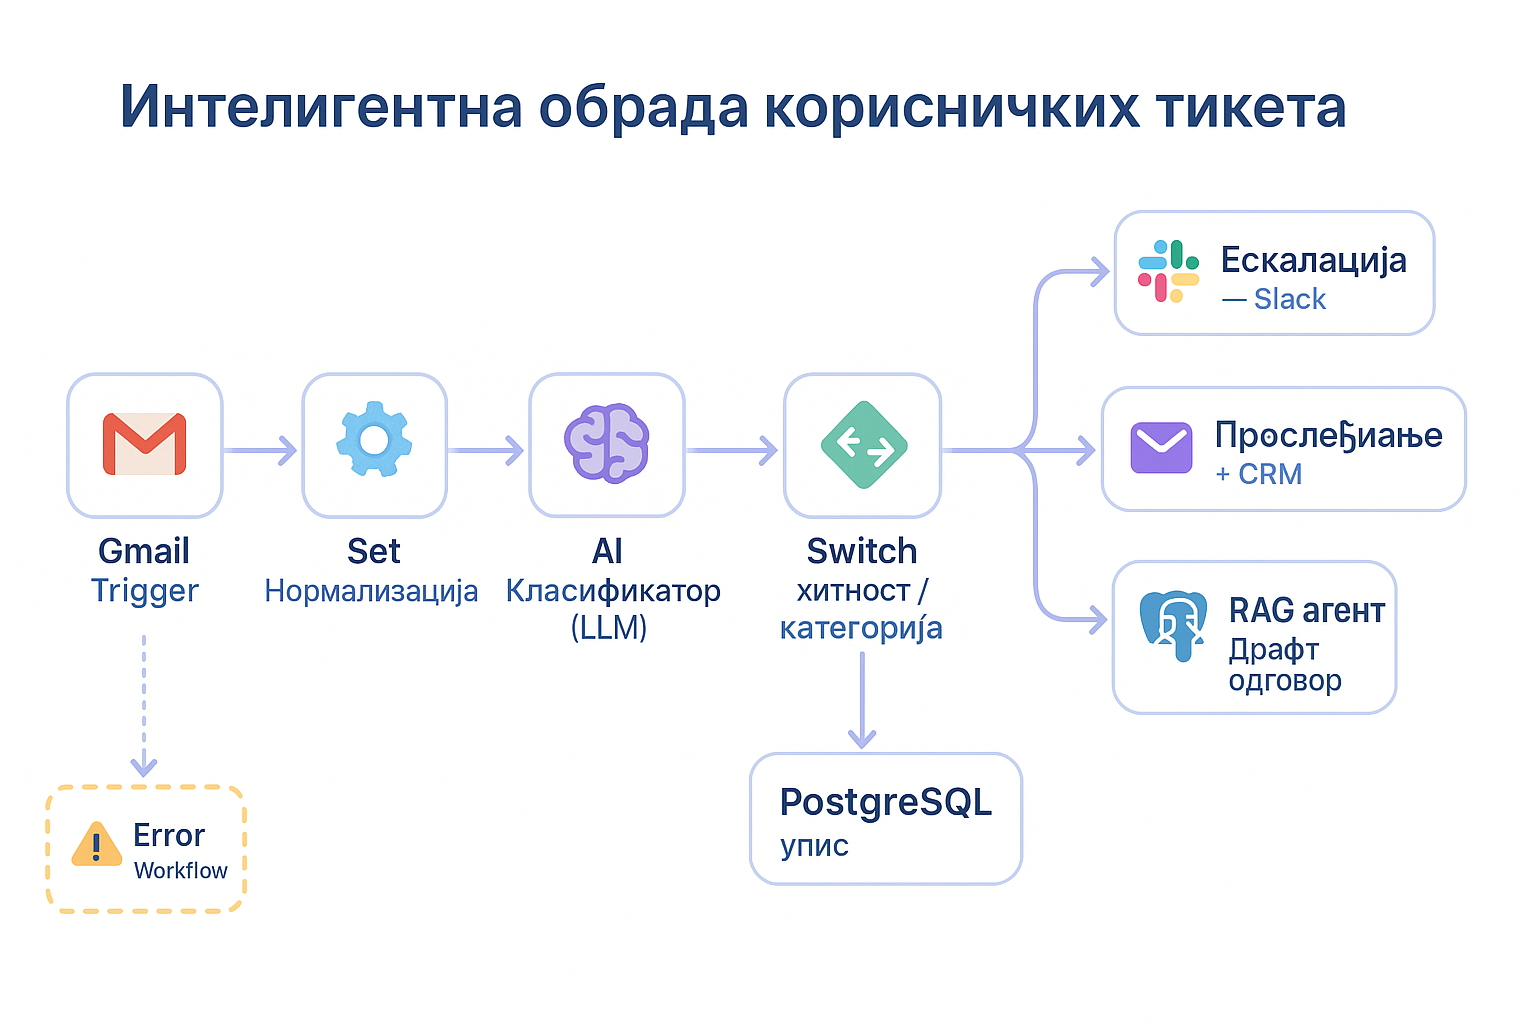
\includegraphics[width=0.95\textwidth]{slike/04/n8n_ticket_workflow.png}
    \caption{Визуелни приказ радног тока за интелигентну обраду корисничких тикета у \textit{n8n}}
    \label{fig:04-13}
\end{figure}

\subsubsection{Анализа решења}

Представљени пример демонстрира неколико кључних својстава
n8n платформе и општих принципа AI аутоматизације:

\begin{itemize}
    \item \textbf{Композитна интелигенција:} систем користи два
    независна AI агента — један за класификацију, други за
    генерисање одговора — што је у складу са принципом
    специјализације из мулти-агентске парадигме.
    \item \textbf{Структурисани излаз као интеграциона граница:}
    класификациони агент не враћа слободан текст, већ строго
    дефинисан JSON, што омогућава детерминистичко гранање у Switch
    чвору.
    \item \textbf{Human-in-the-loop:} за рутинске случајеве систем
    не преузима пуну одговорност, већ припрема предлог који човек
    одобрава — што је у складу са принципима Guardrails слоја из
    одељка~\ref{sec:tehnicka-infrastruktura}.
    \item \textbf{Отпорност на грешке:} експлицитно дефинисан Error
    Workflow обезбеђује да грешка у једном делу система не доведе
    до губитка корисничких упита.
    \item \textbf{Опсервабилност:} свака извршена инстанца радног
    тока оставља комплетан траг у execution history-ју, чиме се
    омогућава ревизија одлука и континуирано побољшање промптова
    и правила.
\end{itemize}

\subsubsection{Могући правци проширења}

Представљени систем може се постепено надограђивати увођењем
напреднијих компоненти:

\begin{itemize}
    \item додавањем дугорочне меморије агента, чиме систем
    „памти“ историју комуникације са сваким појединачним клијентом,
    \item увођењем евалуационог агента који вреднује квалитет
    генерисаних предлога и аутоматски усавршава промптове,
    \item проширењем на omnichannel сценарије (WhatsApp, web chat,
    позиви претворени у текст кроз STT моделе),
    \item интеграцијом са системом за аутоматску детекцију аномалија
    у оптерећењу и темама, што омогућава проактивно упозоравање
    менаџмента на системске проблеме.
\end{itemize}

Тиме се демонстрира како се релативно једноставан иницијални радни
ток може временом развијати у комплексан, аутономни систем за
подршку одлучивању, без фундаменталне промене основне архитектуре
платформе.

\newpage

% =================================================================================
% POGLAVLJE 6
% =================================================================================
\section{Будућност рада и етички аспекти}

Поред техничких аспеката AI система неопходно је сагледати шире импликације убрзаног развоја и примене AI система заснованих на агентима. Иако су претходна поглавља била фокусирана на техничке аспекте и архитектуралне разлике, стварни домет ове технологије огледа се у њеном утицају на економске структуре, тржиште рада, друштвене односе и етичке оквире доношења одлука. На слици~\ref{fig:04-14} дат је концептуални приказ кључних оса одговорног увођења AI система у радно окружење, као и трансформације улоге човека из непосредног извршиоца у надзорника и архитекту аутономних система.

\begin{figure}[h!]
    \centering
    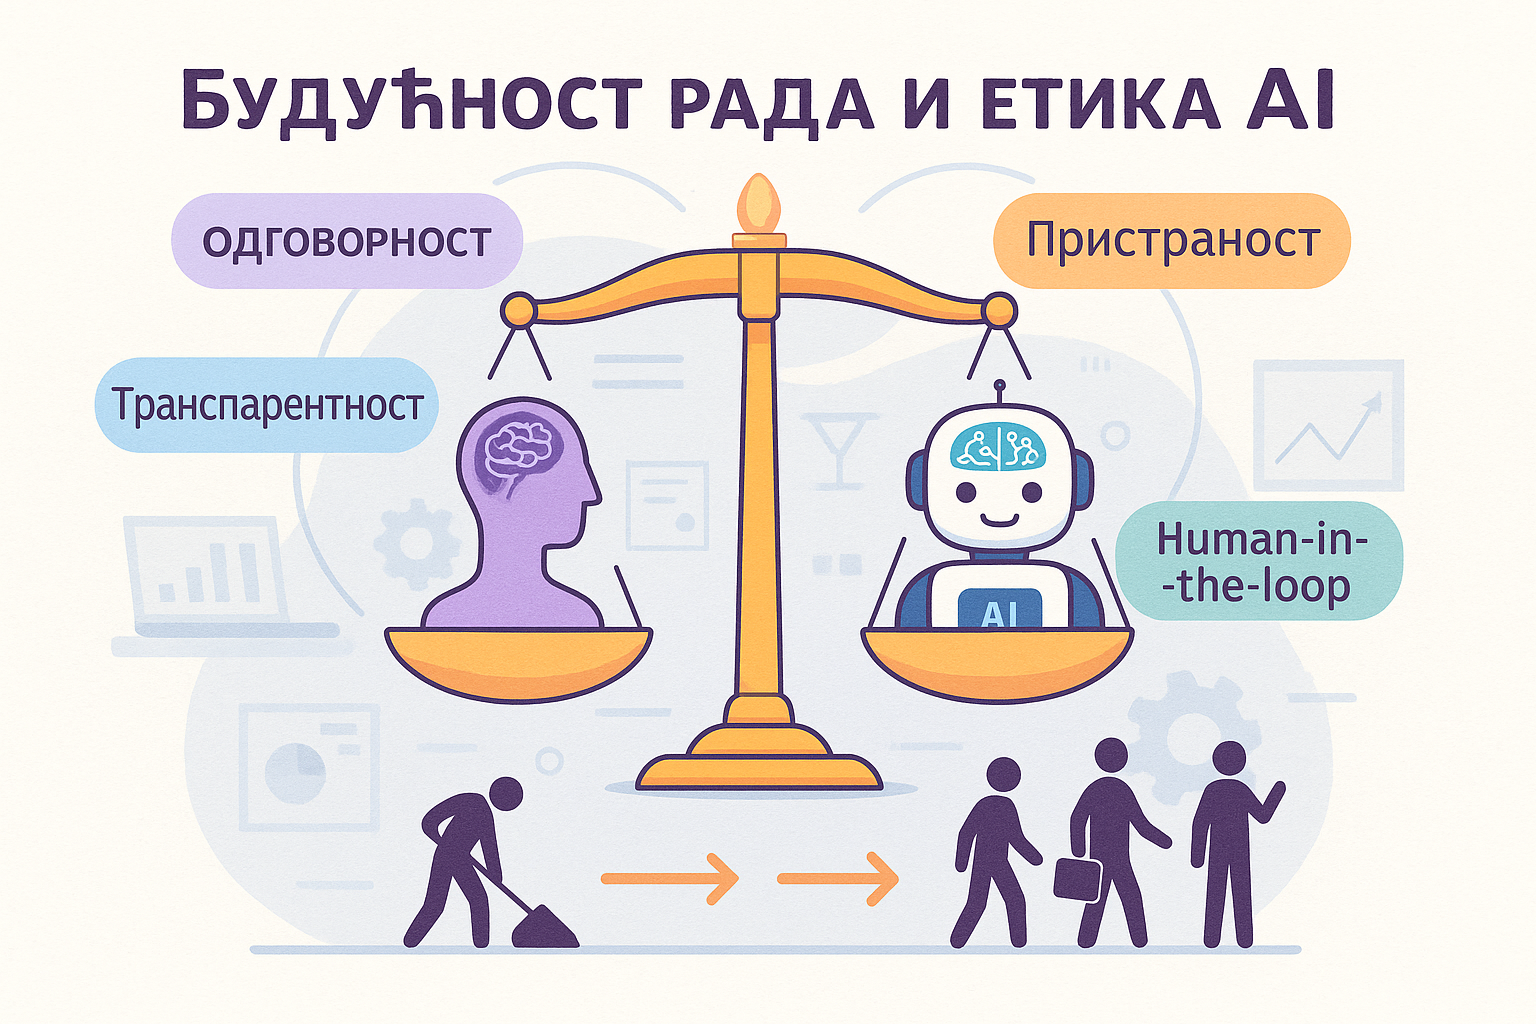
\includegraphics[width=0.85\textwidth]{slike/04/etika_buducnost_rada.png}
    \caption{Етички оквир и трансформација улоге човека у ери AI агената}
    \label{fig:04-14}
\end{figure}

Развој аутономних и полуаутономних AI агената не представља само технолошки напредак, већ и дубоку промену парадигме рада и организације друштва~\cite{schwab2017,frey2017}. У том контексту, AI се више не посматра искључиво као алат, већ као активни учесник у производњи вредности, доношењу одлука и управљању процесима.

\subsection{Економска предвиђања и продуктивност}

Један од најчешће истицаних макроекономских ефеката примене AI агената јесте драстичан раст индивидуалне продуктивности. Аутономни системи омогућавају да мали тимови, па чак и појединци, управљају процесима који су до недавно захтевали комплексне хијерархије, вишеслојне организационе структуре и значајне људске ресурсе.

AI агенти преузимају улоге аналитичара, оператера, планера и извршилаца, чиме се смањују трансакциони трошкови, убрзава доношење одлука и повећава брзина иновација. Овакав модел рада отвара простор за појаву изузетно агилних организација са минималним бројем запослених, али са диспропорционално великим економским утицајем.

Међутим, овакав раст продуктивности носи и ризике. Економска вредност се све више концентрише око власника технологије, података и инфраструктуре, што може довести до продубљивања неједнакости између различитих друштвених група, региона и држава. У одсуству адекватних регулаторних и редистрибутивних механизама, користи од AI револуције могу остати ограничене на узак слој актера.

\subsection{Трансформација тржишта рада}

Аутоматизација заснована на AI агентима неминовно доводи до трансформације структуре тржишта рада~\cite{frey2017,schwab2017}. Традиционална радна места, заснована на понављајућим, процедуралним или административним задацима, постају посебно рањива. Истовремено, не долази до потпуног нестанка људског рада, већ до његове дубоке реконфигурације.

Улога човека се постепено помера са директног извршавања задатака ка:
\begin{itemize}
    \item надзору аутономних система,
    \item дефинисању циљева и ограничења,
    \item евалуацији квалитета и последица одлука,
    \item управљању изузетним ситуацијама и грешкама.
\end{itemize}

Другим речима, човек постаје \textit{arhitekta sistema} и \textit{чувар смисла}, док AI преузима оперативни део рада. Ова промена захтева нове компетенције и континуирано прилагођавање образовних система.

Појављују се нове професионалне улоге и вештине:
\begin{itemize}
    \item \textbf{Промпт инжењеринг:} способност прецизног формулисања захтева, ограничења и циљева за AI системе~\cite{sahoo2024prompt};
    \item \textbf{Оркестрација агената:} дизајнирање и управљање интеракцијама између више аутономних агената у комплексним токовима рада;
    \item \textbf{AI надзор и евалуација:} процена поузданости, робусности и граница аутономних система;
    \item \textbf{Интердисциплинарна писменост:} разумевање како техничких, тако и друштвених и правних импликација AI одлука.
\end{itemize}

Истовремено, постоји реална опасност од структурне незапослености у секторима који не успеју да се прилагоде овом прелазу, што додатно наглашава потребу за активним политикама преквалификације и социјалне заштите.

\subsection{Етички аспекти аутономних AI система}

Са порастом аутономије AI агената, етичка питања постају централна тема њихове примене~\cite{hleg2019,bender2021}. Кључни изазов лежи у чињеници да AI системи доносе одлуке које могу имати директне последице по појединце и друштво, често на основу пробабилистичких и нетранспарентних модела~\cite{russell2020}.

Једно од основних етичких питања односи се на одговорност. У ситуацијама када AI агент направи грешку или проузрокује штету, поставља се питање: ко сноси одговорност — дизајнер система, корисник, организација или сам систем као аутономни ентитет? Тренутни правни оквири углавном нису прилагођени оваквим сценаријима.

Други кључни аспект је пристрасност~\cite{bender2021}. AI системи уче из података који рефлектују постојеће друштвене неједнакости, што може довести до репродукције или чак амплификације дискриминаторних образаца. Без континуираног етичког надзора, аутономни агенти могу доносити систематски неправедне одлуке, нарочито у областима као што су запошљавање, кредитирање или правосуђе~\cite{hleg2019}.

Трећи изазов представља транспарентност и објашњивост. Како системи постају сложенији и дистрибуиранији (посебно у мулти-агентским архитектурама), све је теже реконструисати ланац одлука који је довео до одређеног исхода. Ово отежава ревизију, регулацију и изградњу поверења између људи и AI система.

На дужи рок, широка примена AI агената може довести до редефинисања основних друштвених категорија рада, вредности и идентитета. Ако продуктивност постане готово независна од људског рада, друштва ће се суочити са питањима прерасподеле богатства, редефинисања радног времена и саме сврхе рада у људском животу.

Поставља се и питање когнитивне зависности: ослањање на AI агенте за планирање, доношење одлука и решавање проблема може довести до ерозије одређених људских вештина. Из тог разлога, будући системи морају бити дизајнирани не само као замена за људски рад, већ и као алат за његово унапређење.

Закључно, будућност рада у ери AI агената не зависи искључиво од технолошког напретка, већ од начина на који друштво одлучи да ову технологију интегрише. Баланс између ефикасности, праведности и људске аутономије представљаће један од кључних изазова савременог доба.

Важно је напоменути да AI аутоматизација није само технолошки тренд, већ фундаментална промена у начину организације рада. Прелазак са линеарних скрипти на аутономне агенте омогућава ниво продуктивности и скалабилности који је раније био незамислив.



% =================================================================================
% PRILOG
% =================================================================================

\section{Литература}
\printbibliography[heading=none]
